\subsection{Major Reducible Background
\label{sec:faketaubkg}}

The major reducible background comes from events with jets misidentified as hadronic taus. This background has contributions from the \W + jets, \Z + jets, \ttbar, and QCD multijet processes. The contribution from \W + jets, \Z + jets, and \ttbar is estimated from observed data by measuring the misidentification probability or ``fake rate''. The QCD events contain mostly gluon jets, while the events from the other processes contain mostly quark jets. Gluon jets tend to be wider than quark jets and to have higher multiplicity, with a correspondingly lower energy per particle. Therefore, gluon jets are less likely to pass isolation and therefore have a lower fake rate. The fake rate used in this estimation is measured in a control region that is appropriate for the quark jet processes. Therefore, this fake rate cannot produce an accurate estimate of the contribution from QCD. This contribution is estimated using a same-sign/opposite-sign (SS/OS) method, which is described in Sec. \ref{sec:qcdbkg}. The contribution from QCD is non-negligible only in the \etau channel of the leptoquark search. In this case, the reconstructed electron is also a misidentified jet. A jet is much less likely to be misidentified as a muon, so QCD does not contribute in the \mutau channel. In the top squark search, the high jet multiplicity requirement eliminates any significant contribution from QCD.

The probability for a jet to be misidentified as a hadronic tau is measured from the observed data in a \Zmm + jets control region. The selection of the primary muon uses the same criteria as the \mutau channel in the signal region. The second muon is selected using the loose working point for identification and isolation, along with looser kinematic cuts. The two muons are required to have the same vertex, opposite charges, and a separation of $\Delta R > 0.5$. This ensures the orthogonality of the control region because of the opposite-sign additional lepton veto in the signal region. The selection of hadronic tau candidates, which are misidentified jets in the \Zmm + jets control region, uses the same identification, discriminator working points, and kinematic cuts as the signal selection. However, the hadronic tau candidates are not required to be isolated, as the isolation variable is used to compute the fake rate. All selected hadronic taus must originate from the same vertex as the two muons and must be separated from each muon with $\Delta R > 0.5$. A cut on the invariant mass of the two muons is also applied, $M_{\mu\mu} > 50\GeV$, in order to match the generation of the simulated \Z + jets samples.

This selection produces a control region which consists of $95\%$ \Z + jets events. The simulated \Z + jets sample is normalized to the yield from the observed data, with the yield from the other simulated backgrounds subtracted. The normalization factor is $N[\text{data}~-~\text{other MC}]/N[\text{Z + jets}] = 0.924 \pm 0.003$, calculated using the range $70 < M_{\mu\mu} < 110\GeV$. Figure \ref{Bkg:fig:Zregion} shows the dimuon mass $M_{\mu\mu}$ and the multiplicity of extra jets, which are not misidentified as hadronic taus, in the \Zmm + jets control region. Good agreement is seen between data and simulation, demonstrating the validity of the control region. The majority of events contain no extra jets, but an appreciable percentage, around $40\%$, contain one or more extra jets.

\begin{figure}[hbt]
  \begin{center}
    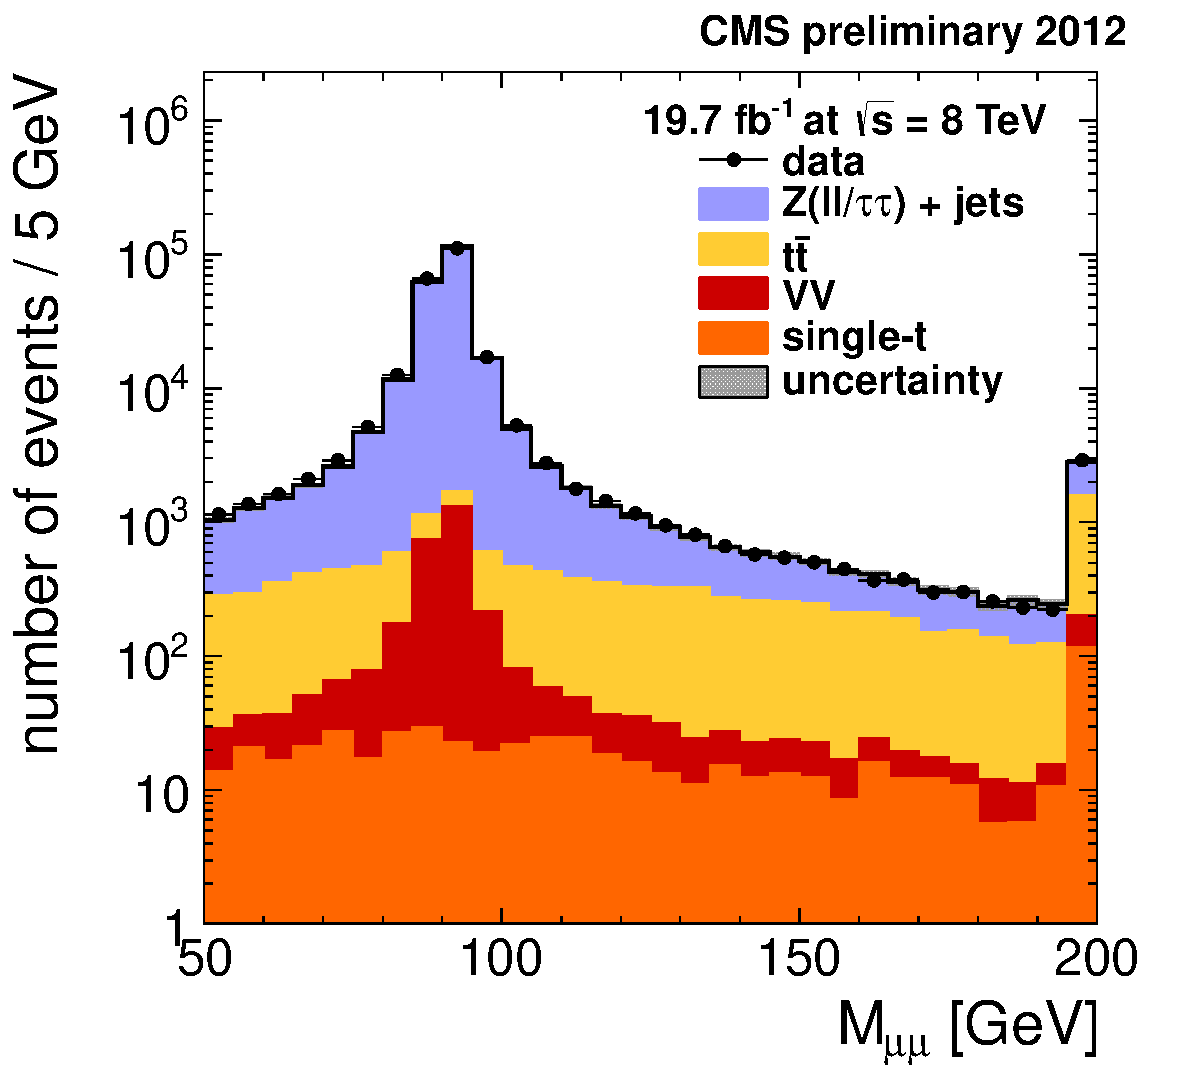
\includegraphics[width=0.49\textwidth]{figures/bkgEstim/massdimuon.pdf}
    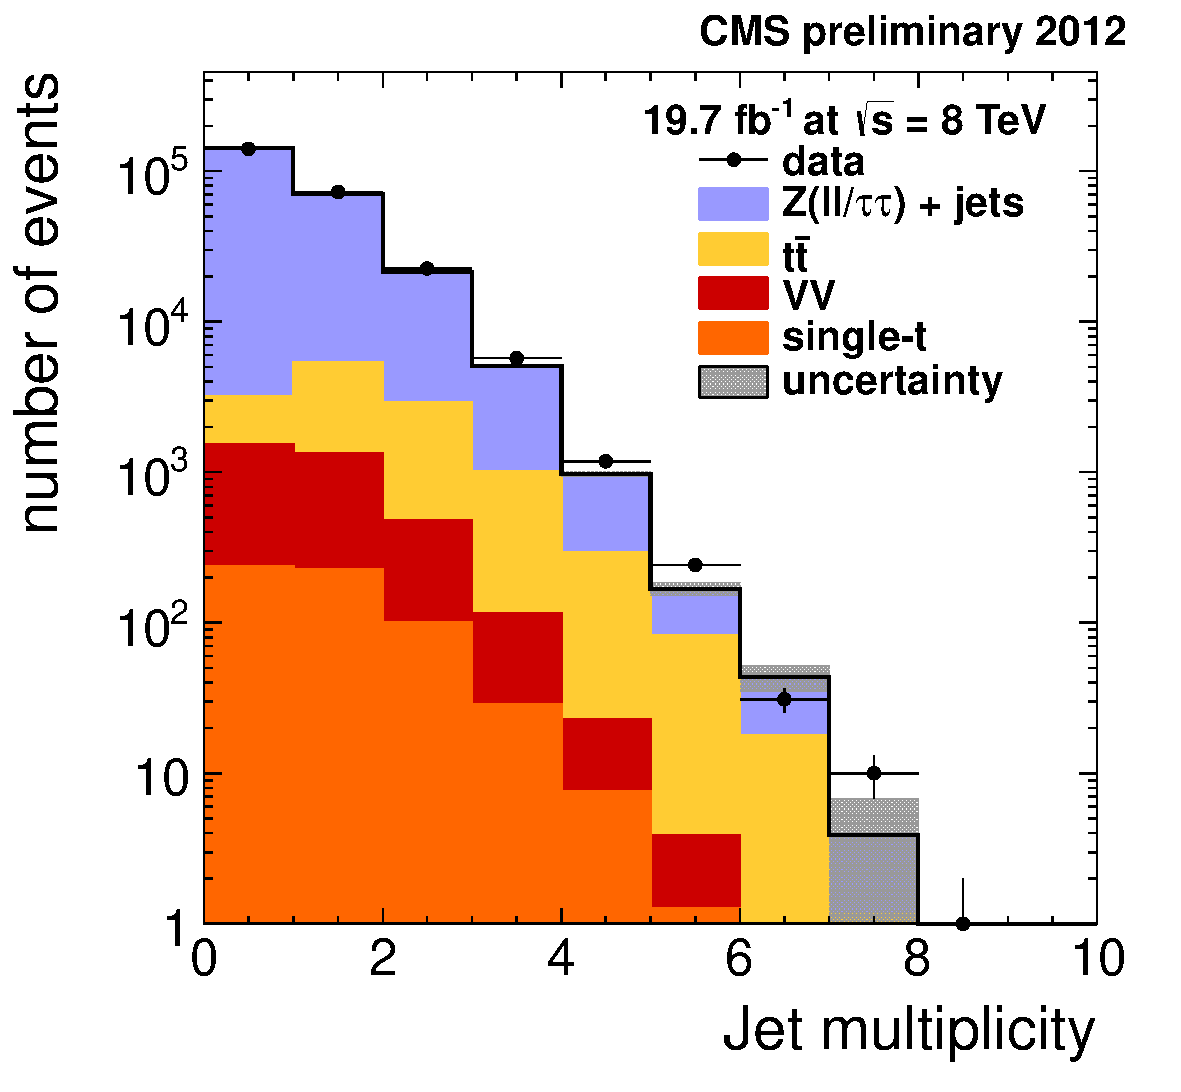
\includegraphics[width=0.49\textwidth]{figures/bkgEstim/njet.pdf}
    \caption{Comparison of observed data and simulation in the \Zmm + jets control region for $M_{\mu\mu}$ (left) and multiplicity of extra jets, which are not misidentified as hadronic taus (right). \label{Bkg:fig:Zregion}}
  \end{center}
\end{figure}

All hadronic tau candidates in the \Zmm + jets control region are considered when calculating the fake rate. These hadronic tau candidates are misidentified jets which pass all selection requirements for hadronic taus, except that isolation is not required. The subset of these candidates which also pass the isolation requirement would be fully misidentified as hadronic taus. The fake rate is therefore the rate at which the hadronic tau candidates pass the isolation requirement. It is parameterized as a function of the transverse momentum of the tau candidates, as shown in Eq. \eqref{Bkg:eq:FR}:
\begin{equation} f(\pt) = \frac{N_{\text{iso}~\tau}^{(\Zmm)}(\pt)}{N_{\text{all}~\tau}^{(\Zmm)}(\pt)} \label{Bkg:eq:FR} \end{equation}

%When calculating the fake rate from the observed data, the contribution from the residual backgrounds is subtracted from both the numerator and the denominator of Eq. \eqref{Bkg:eq:FR}. The residual backgrounds include the diboson and single top processes. The fake rate from the simulation includes both the \Z + jets and \ttbar contributions. The \ttbar contribution is included in the simulated fake rate rather than in the residual backgrounds because its contribution is enhanced in events with extra jets. Such events more closely resemble the main region where at least two jets are required. The observed data and simulated fake rates calculated from all \Zmm + jets events, from events with one or more extra jets, and from events with two or more extra jets are shown in Fig. \ref{Bkg:fig:fakerate}. The fake rate calculated from all \Zmm + jets events is called the inclusive fake rate, since it includes all events regardless of the number of extra jets.

When calculating the fake rate from the observed data, the contribution from the residual background is subtracted from both the numerator and the denominator of Eq. \eqref{Bkg:eq:FR}. The residual background consists of 4\% \ttbar events, 1\% diboson events, and 0.2\% single top quark events. The observed data and simulated fake rates calculated from all \Zmm + jets events, from events with one or more extra jets, and from events with two or more extra jets are shown in Fig. \ref{Bkg:fig:fakerate}. The fake rate calculated from all \Zmm + jets events is called the inclusive fake rate, since it includes all events regardless of the number of extra jets.

\begin{figure}[hbt]
  \begin{center}
    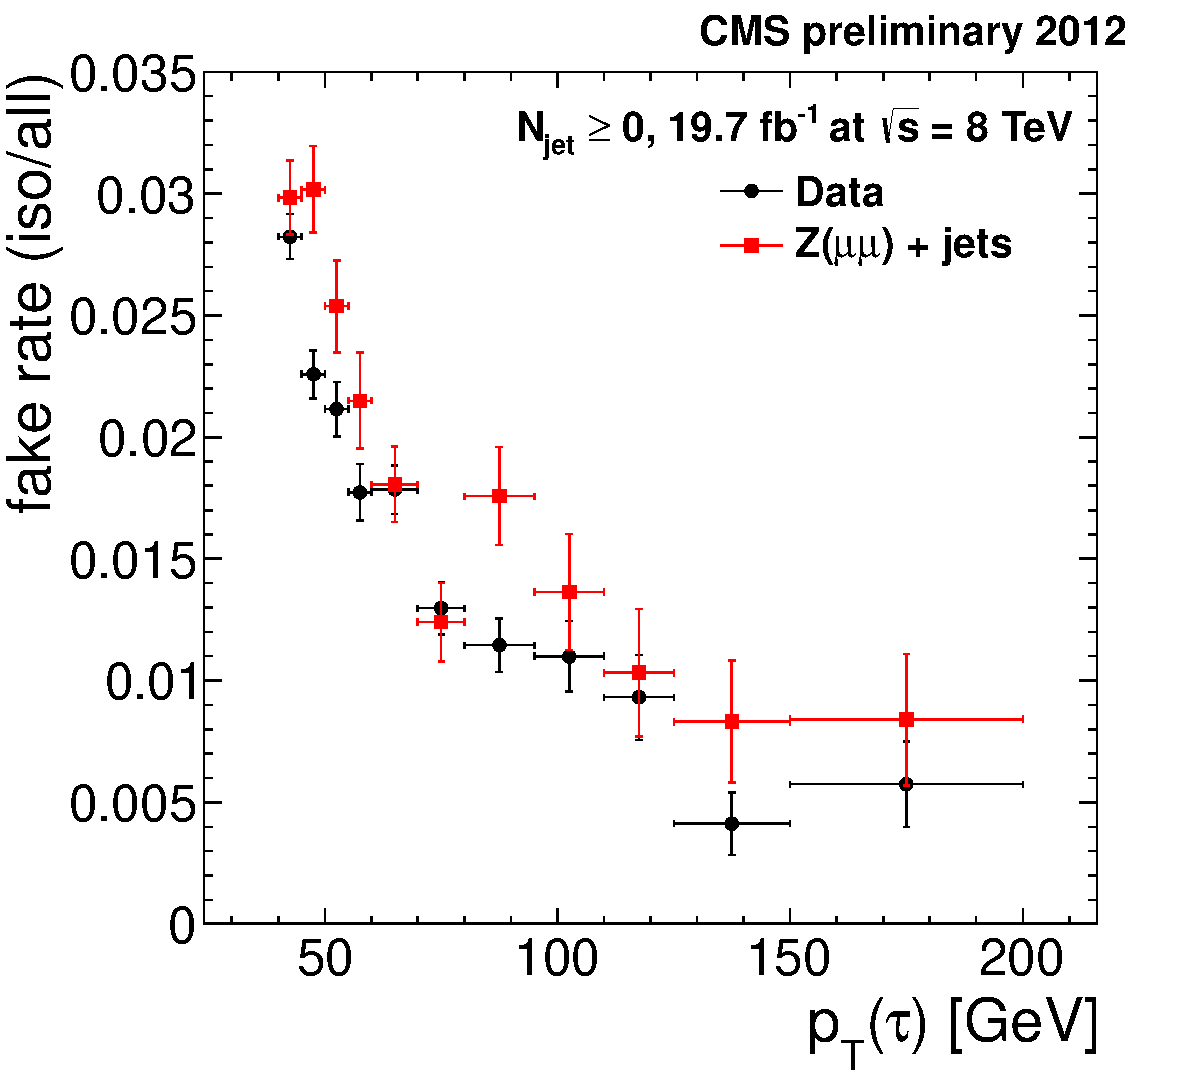
\includegraphics[width=0.32\textwidth]{figures/bkgEstim/tfr_dmc.pdf}
    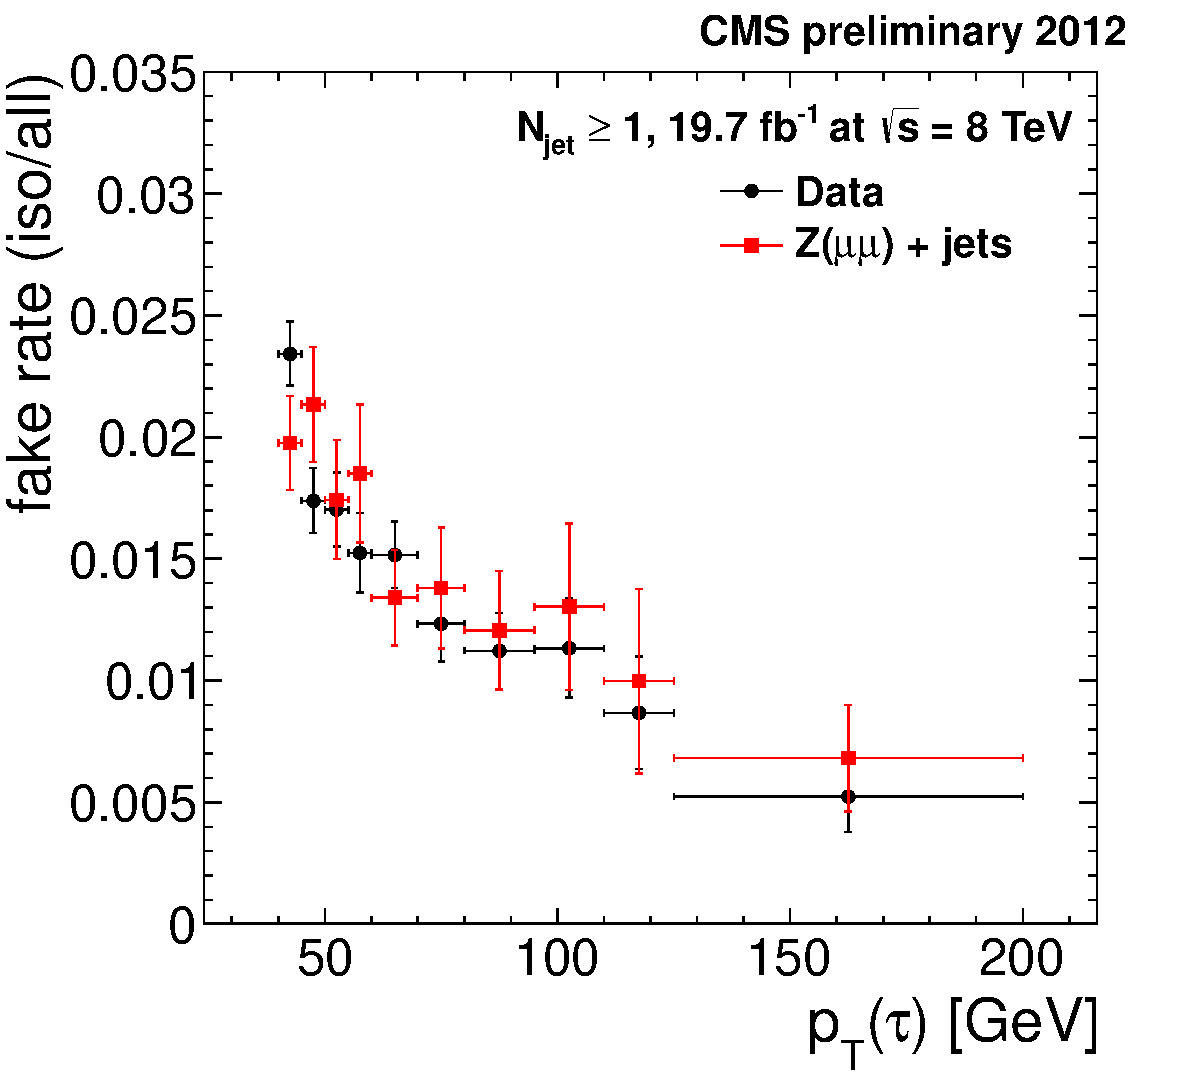
\includegraphics[width=0.32\textwidth]{figures/bkgEstim/tfr_dmc_1jet.pdf}
    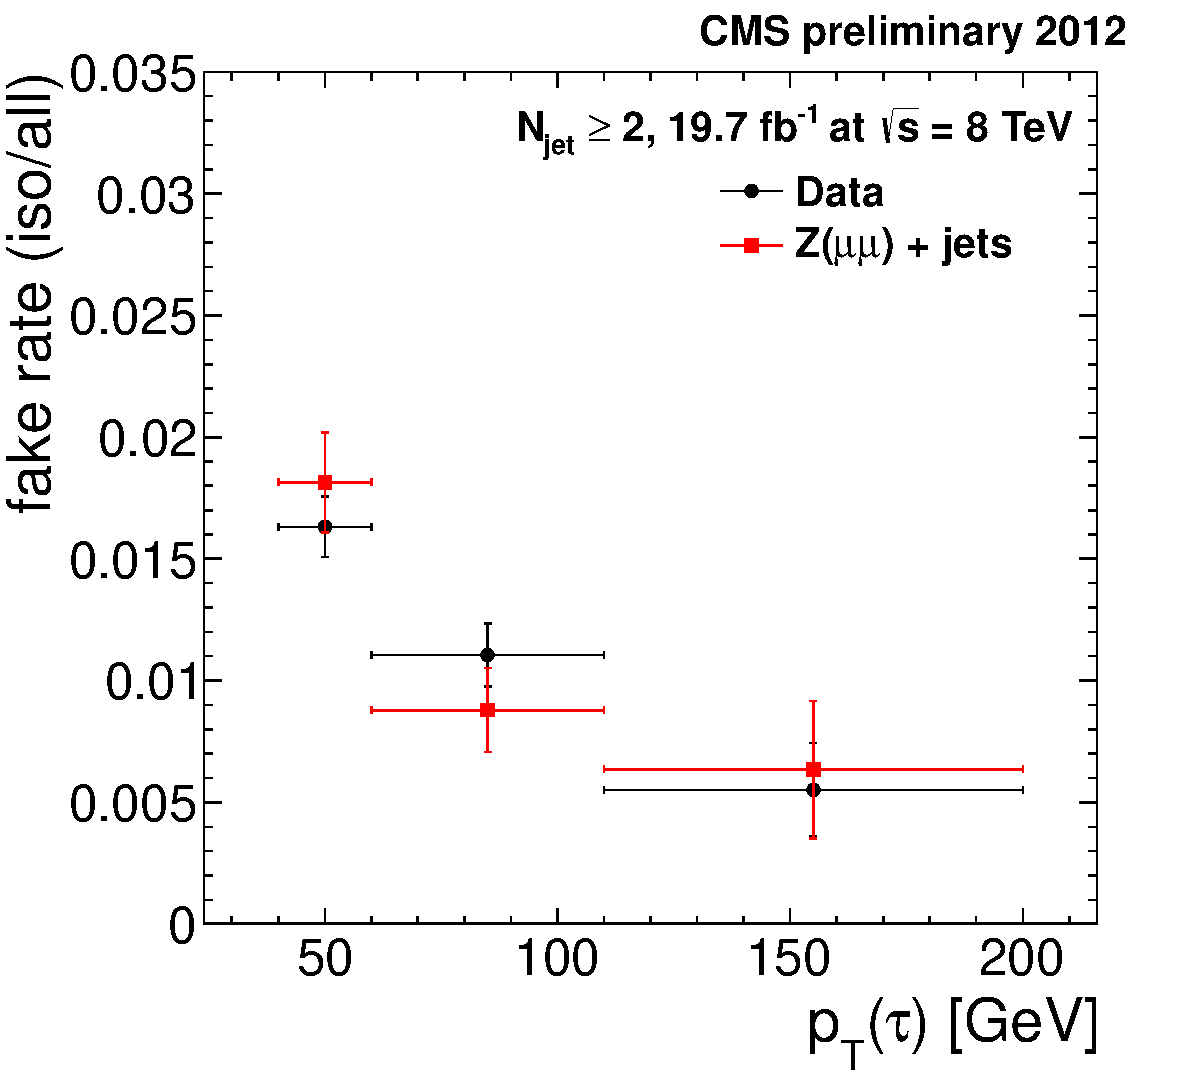
\includegraphics[width=0.32\textwidth]{figures/bkgEstim/tfr_dmc_2jet.pdf}
    \caption{The fake rates measured in the \Zmm + jets control region, using all events (left), only events with one or more extra jets (middle), only events with two or more extra jets (right). \label{Bkg:fig:fakerate}}
  \end{center}
\end{figure}

Events from semileptonic \ttbar decays make up a significant portion of the major reducible background. These events resemble events from the \W + jets process, but with higher jet multiplicities. The relative difference in the fake rate between \Zmm + jets events with $N_{\text{jet}} \geq 1$ and semileptonic \ttbar events is estimated from the simulation and found to be $18\%$. Figure \ref{fig:fakeratettbardiff} shows the simulated fake rates versus hadronic tau \pt and the calculation of the relative difference, which is independent of \pt. This relative difference is multiplied by the percentage of the major reducible background consisting of semileptonic \ttbar events, $35\%$ in the leptoquark search and $95\%$ in the top squark search according to the simulation, and applied as a systematic uncertainty to account for any differences between the types of processes.

\begin{figure}[hbt]
  \begin{center}
    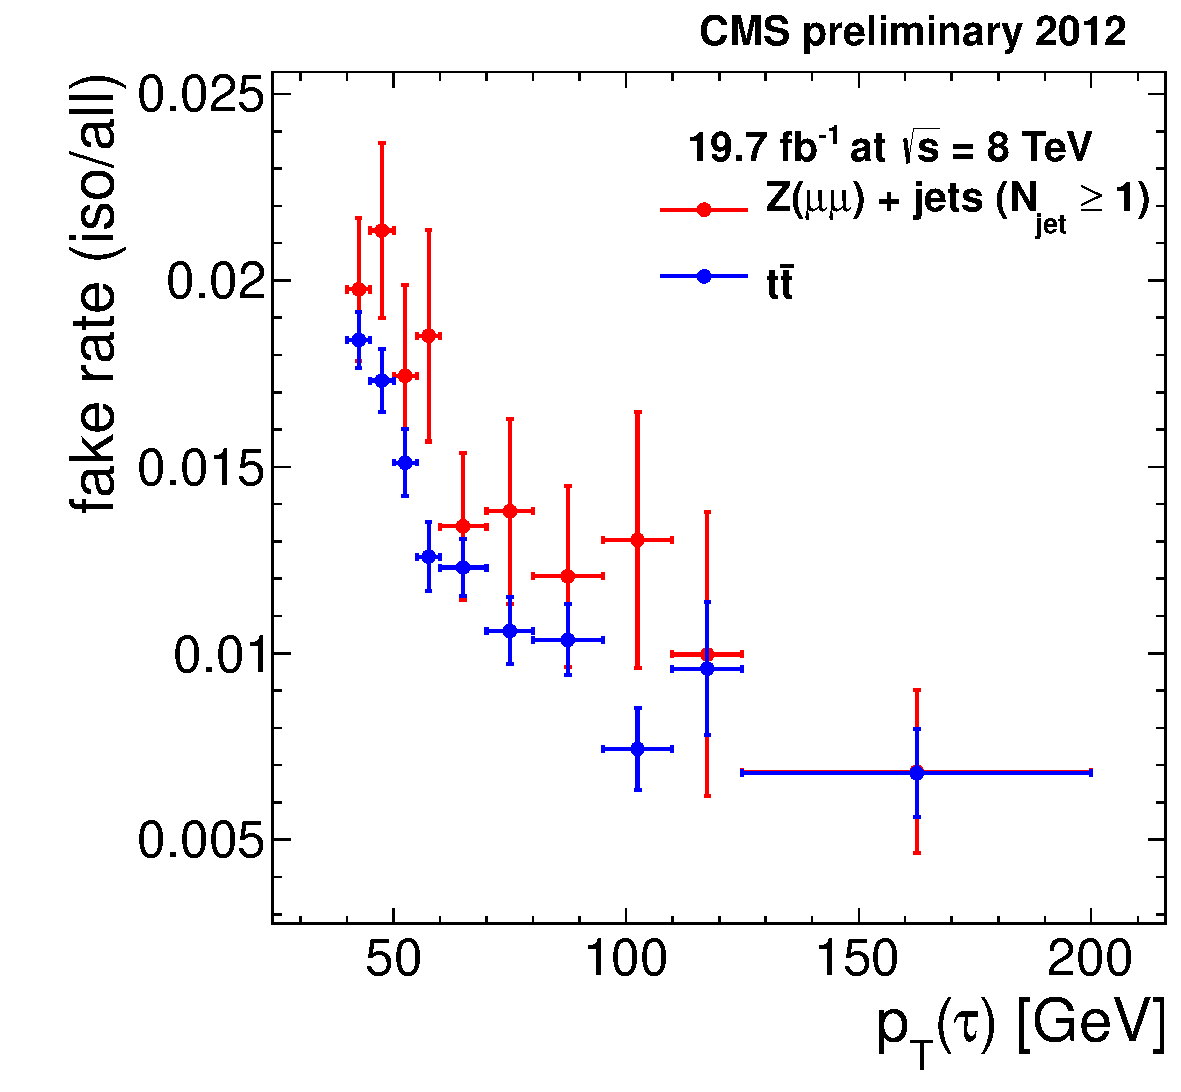
\includegraphics[width=0.32\textwidth]{figures/bkgEstim/ttbar_fr_comp_final.pdf}
    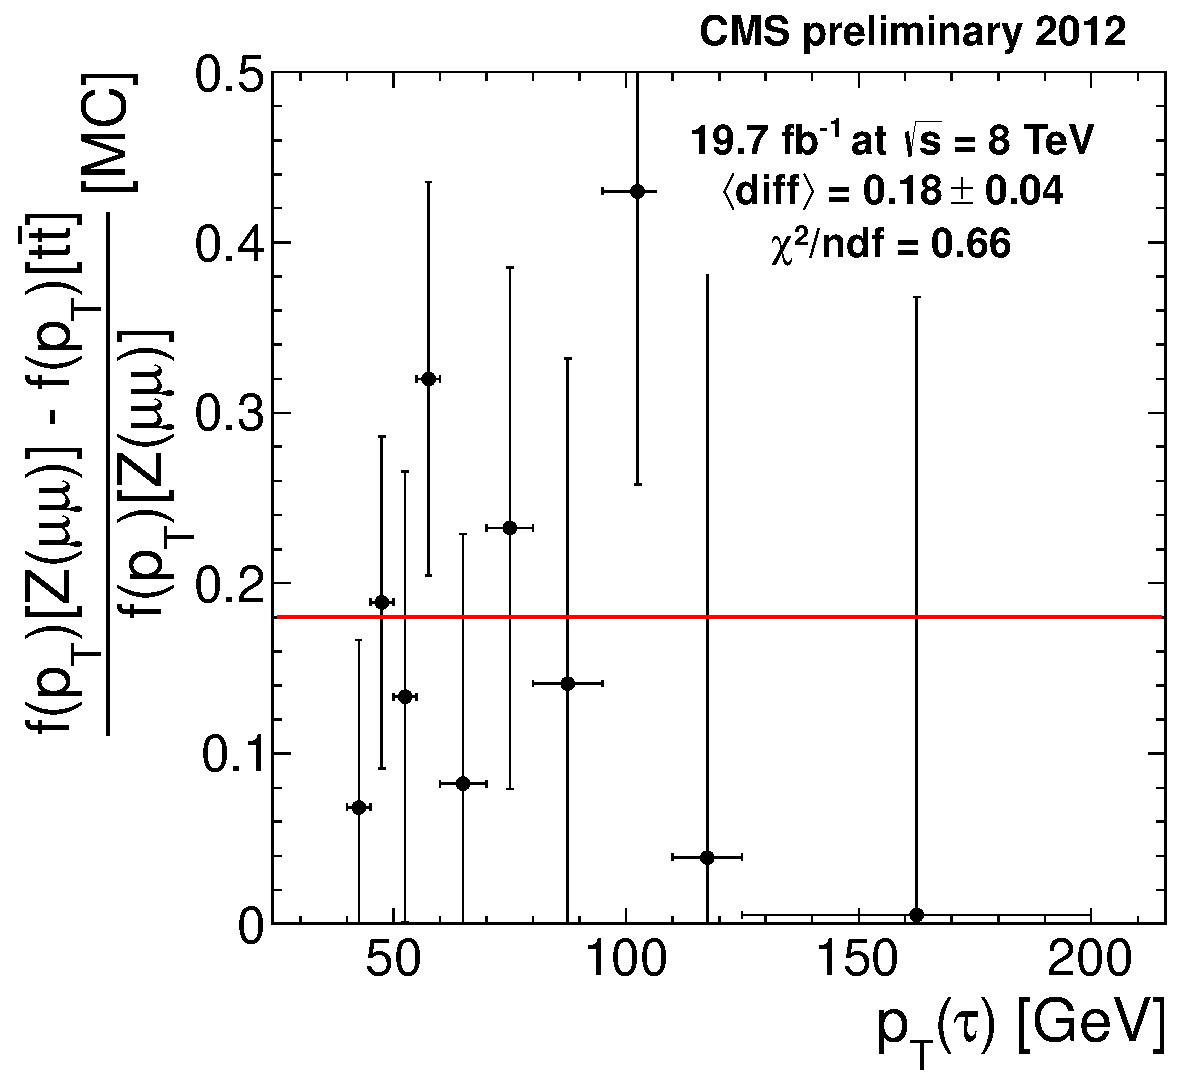
\includegraphics[width=0.32\textwidth]{figures/bkgEstim/tfr_diff_ttbar_incl.pdf}
    \caption{Comparison of the fake rates between simulated \Zmm + jets events with at least one extra jet and simulated semileptonic \ttbar events (left). The difference in the two fake rates is found to be 18\%, independent of the hadronic tau \pt (right). \label{fig:fakeratettbardiff}}
  \end{center}
\end{figure}

To estimate the total yield of the major reducible background in the signal region, a second control region is needed. This control region is defined identically to the signal region, except that events are rejected if any selected hadronic tau passes isolation. This creates an orthogonal region of events in which all selected hadronic taus fail isolation, called the ``anti-isolated'' region. Figures \ref{Bkg:fig:antiiso} and \ref{Bkg:fig:antiiso-lqd321} shows the hadronic tau \pt spectrum and multiplicity in the anti-isolated region for both channels after the leptoquark and top squark final selections, respectively. There is good agreement between observed data and simulated backgrounds in the \mutau channel. In the \etau channel in the leptoquark search, there is an expected disagreement due to a contribution from QCD multijet events in the observed data, which will be addressed. The simulated contributions labeled \W + jets, \Z + jets, and \ttbar contain only events where the hadronic tau candidates are misidentified jets based on matching between the generated and reconstructed particles. The residual background is defined to include events from two categories. The first category consists of events from the diboson and single-top-quark processes, which are not included in the major reducible background. The second category consists of events from the \W + jets, \Z + jets, and \ttbar processes with genuine hadronic taus that fail isolation. The single top quark process contributes 2--5\% depending on the channel and the search, while the other processes contribute less than 1\% each.

\begin{figure}[hbtp]
  \begin{center}
    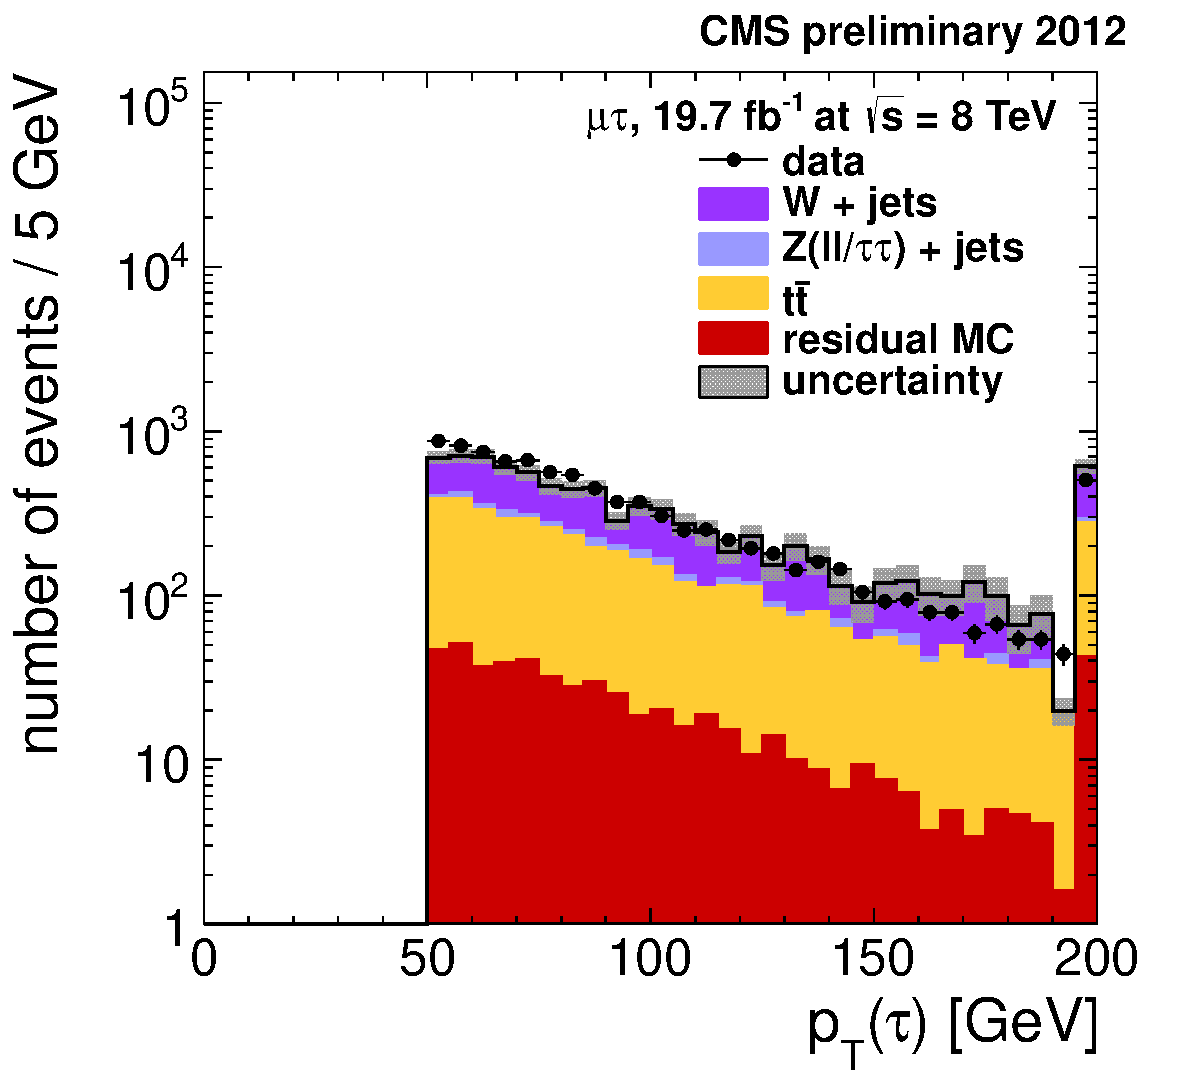
\includegraphics[width=0.49\textwidth]{figures/bkgEstim/pttauantiisoall_mutau.pdf}
    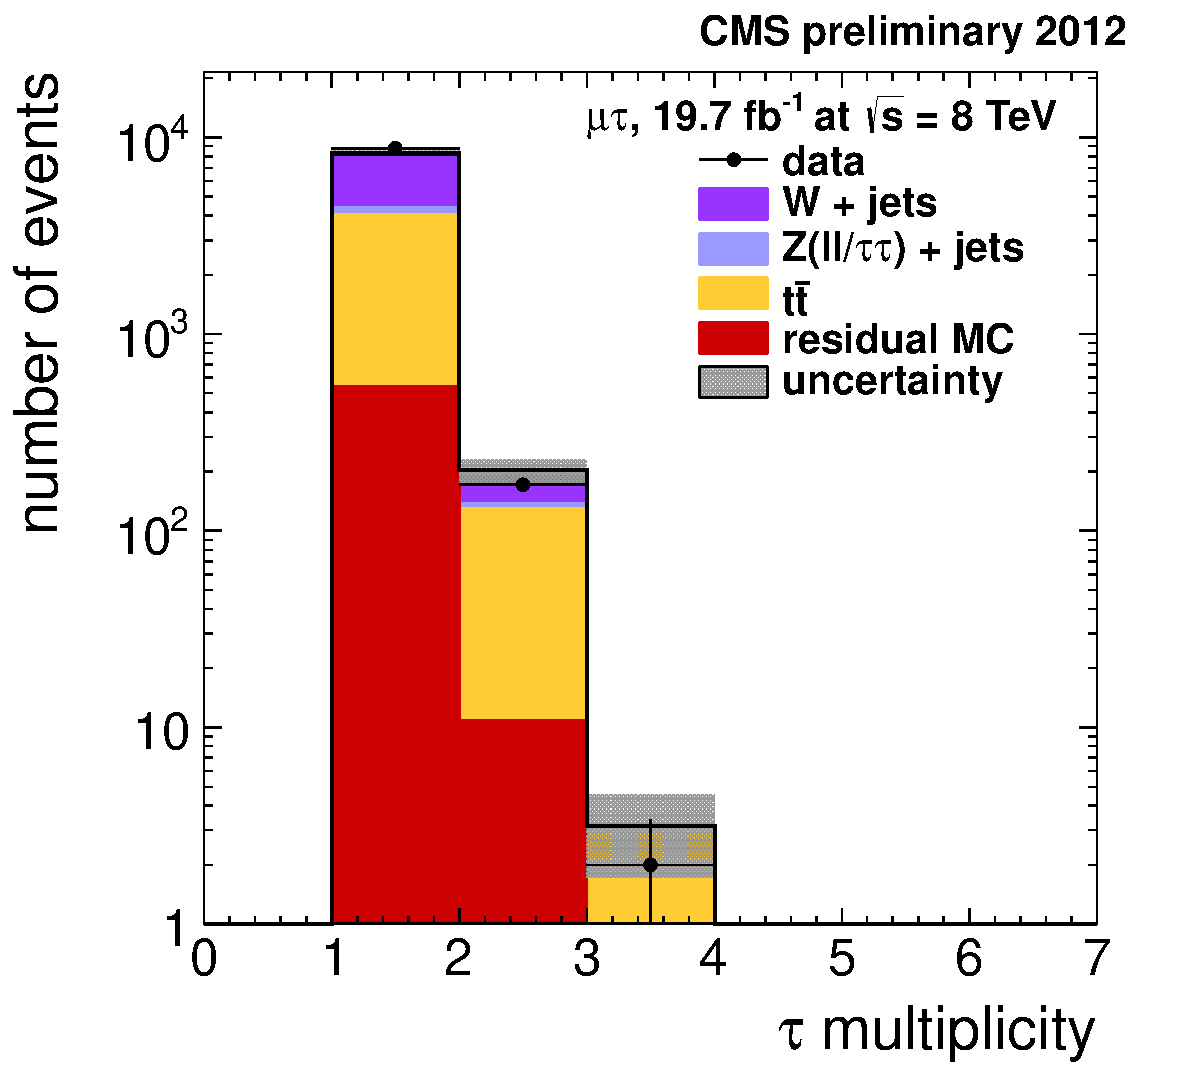
\includegraphics[width=0.49\textwidth]{figures/bkgEstim/ntauantiiso_mutau.pdf} \\
    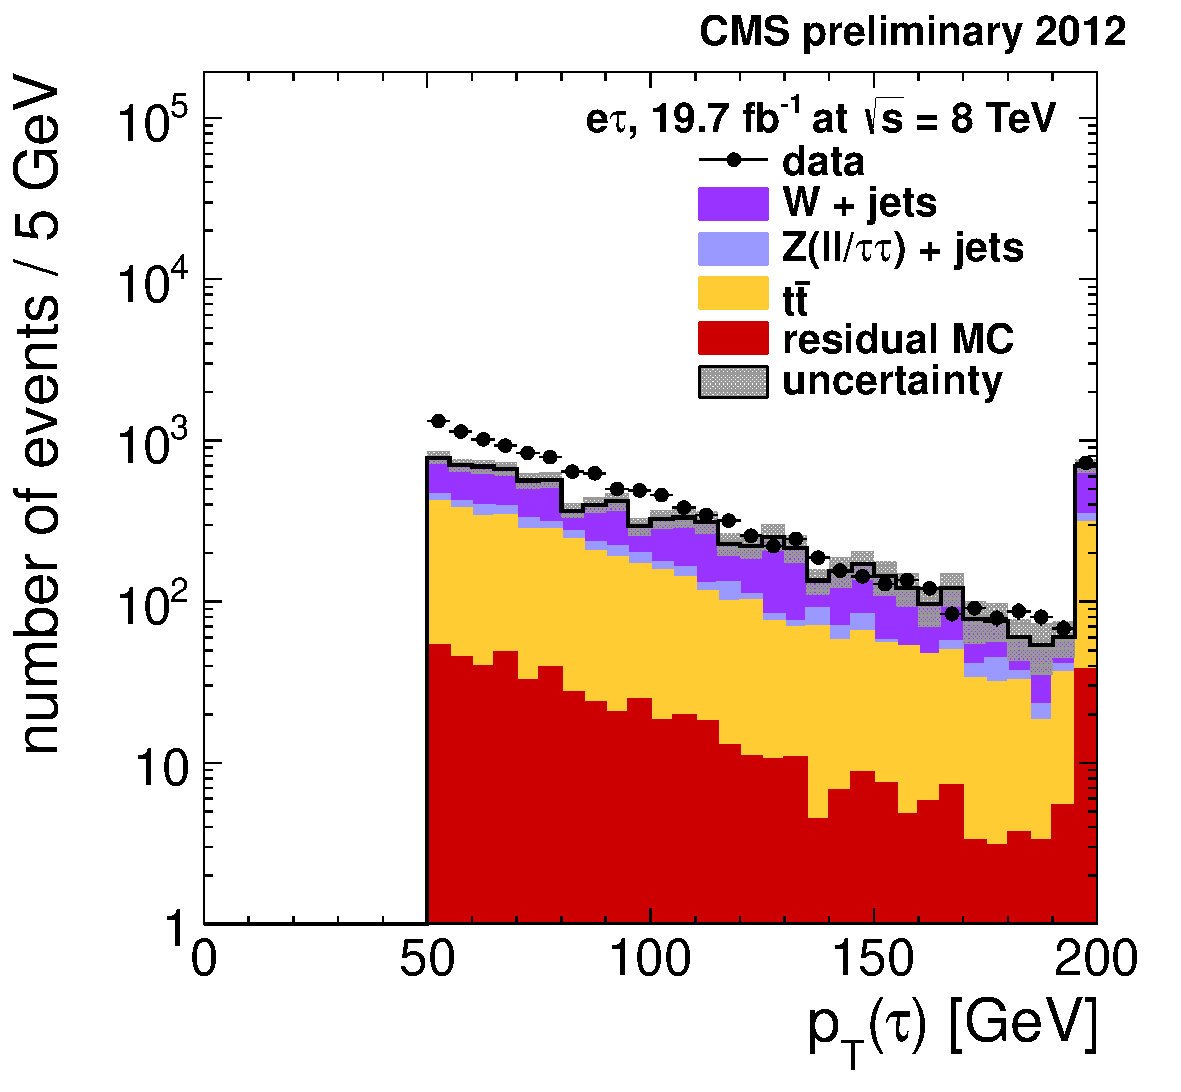
\includegraphics[width=0.49\textwidth]{figures/bkgEstim/pttauantiisoall_etau.pdf}
    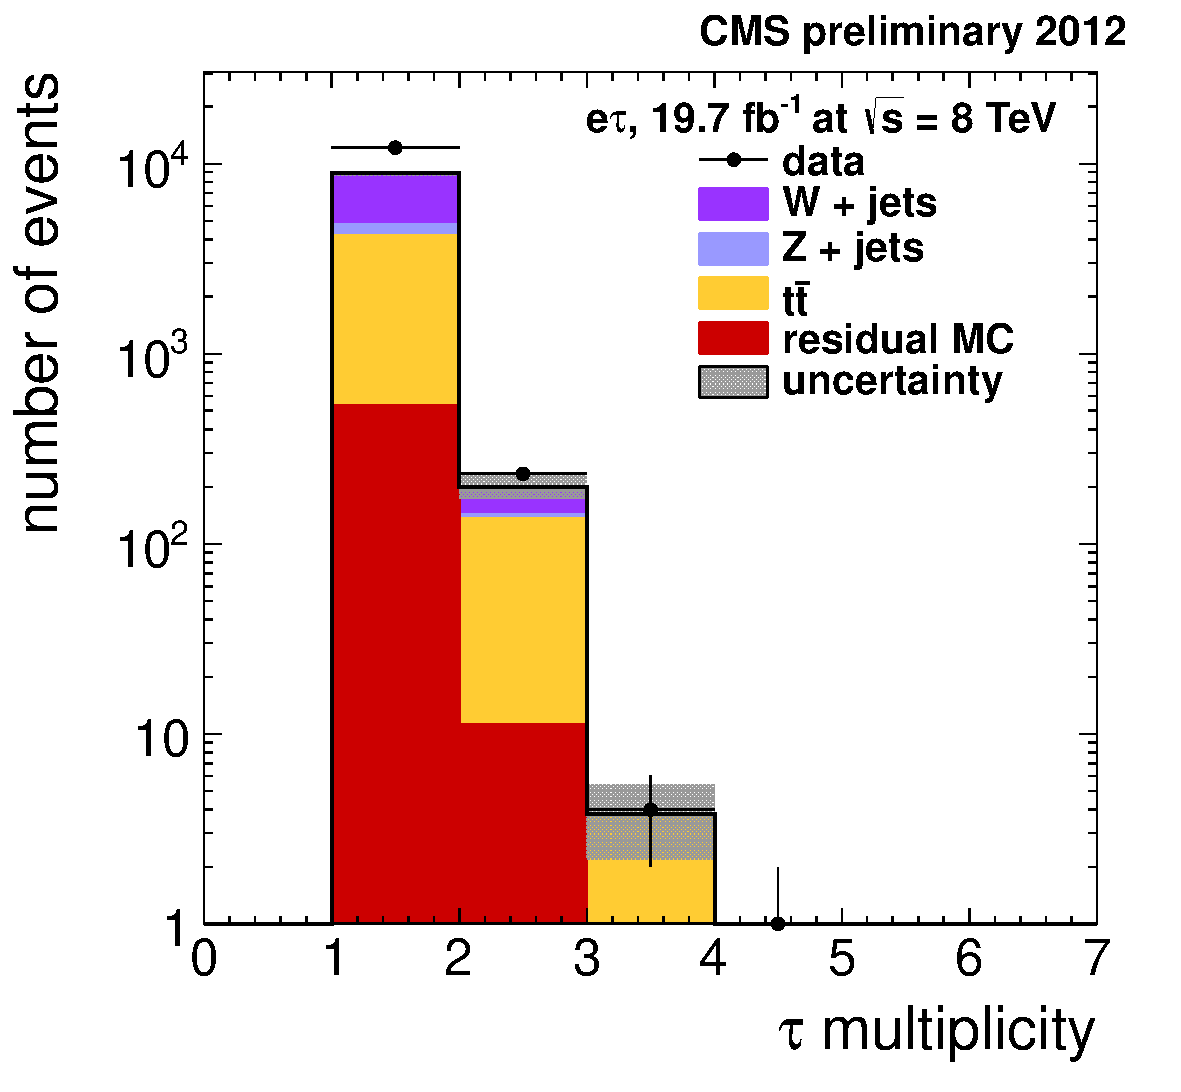
\includegraphics[width=0.49\textwidth]{figures/bkgEstim/ntauantiiso_etau.pdf} 
    \caption{Plots of the anti-isolated control region after the leptoquark final selection, showing the hadronic tau \pt spectrum (left) and multiplicity (right) in the \mutau channel (top) and the \etau channel (bottom). \label{Bkg:fig:antiiso}}
  \end{center}
\end{figure}

\begin{figure}[hbtp]
  \begin{center}
    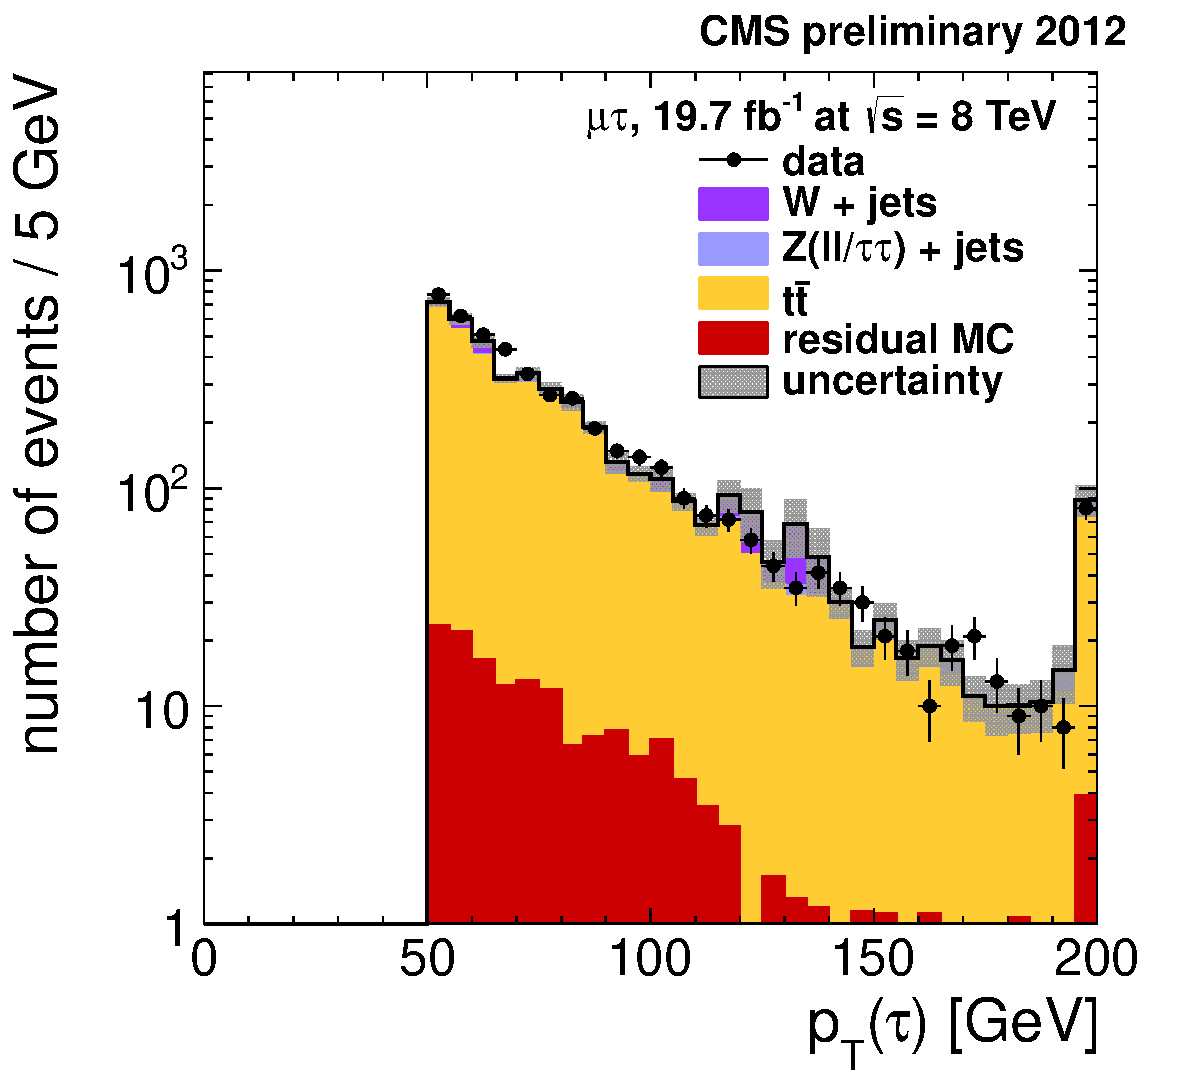
\includegraphics[width=0.49\textwidth]{figures/bkgEstim/pttauantiisoall_mutau_lqd321.pdf}
    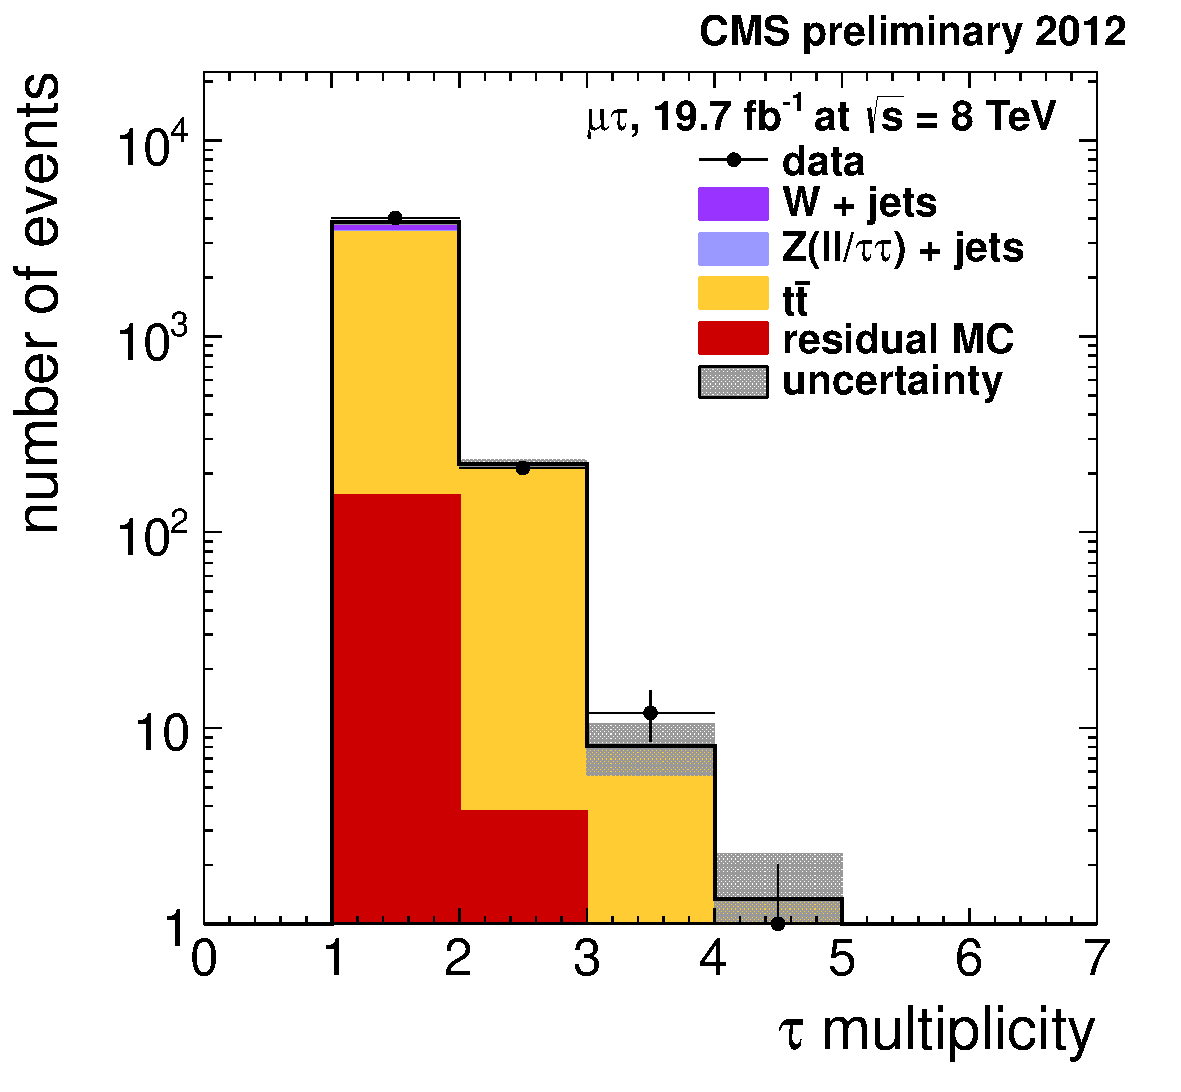
\includegraphics[width=0.49\textwidth]{figures/bkgEstim/ntauantiiso_mutau_lqd321.pdf} \\
    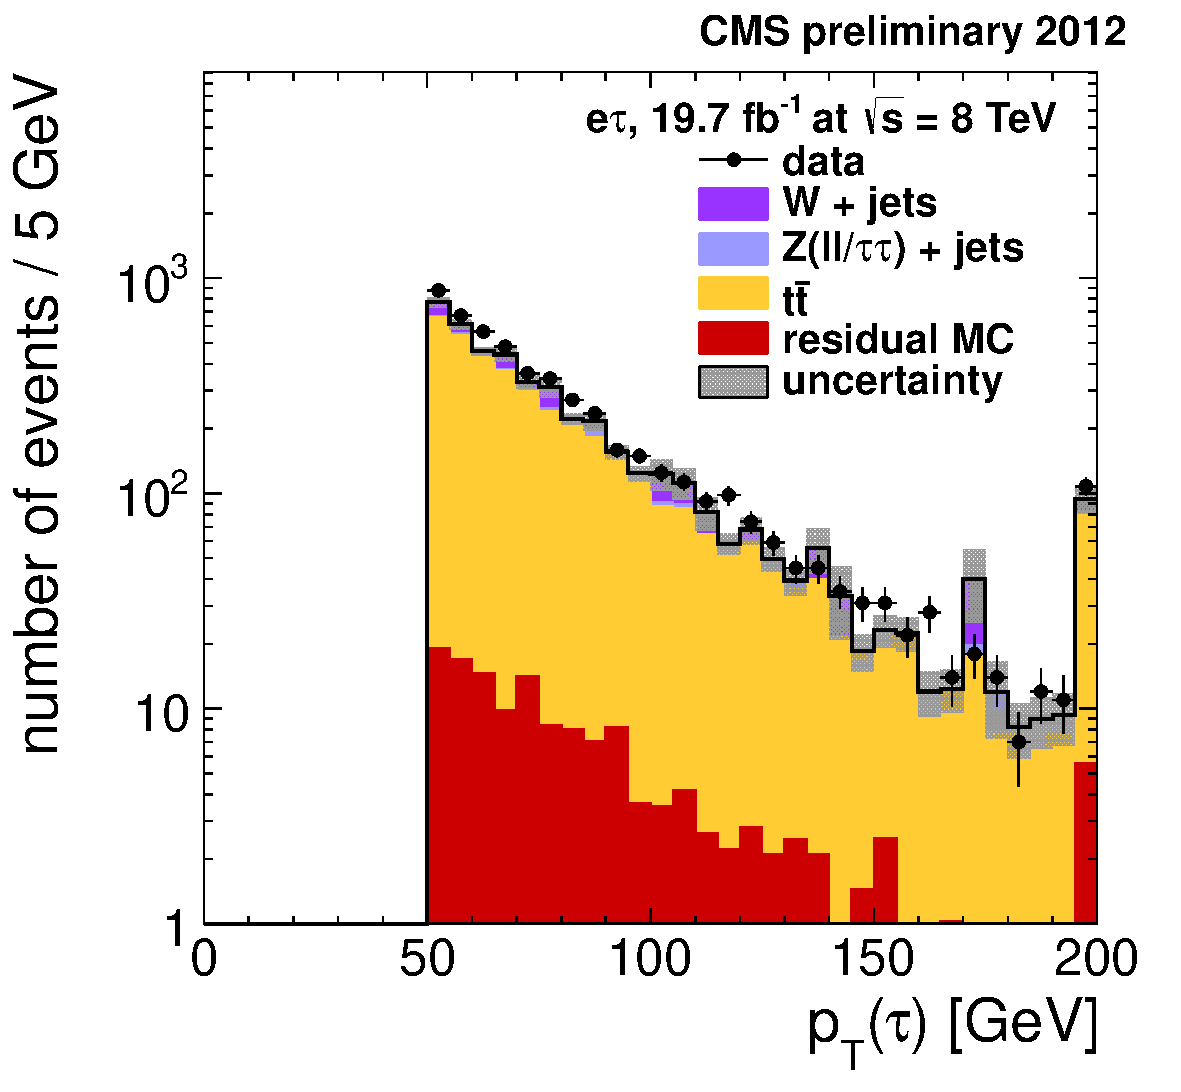
\includegraphics[width=0.49\textwidth]{figures/bkgEstim/pttauantiisoall_etau_lqd321.pdf}
    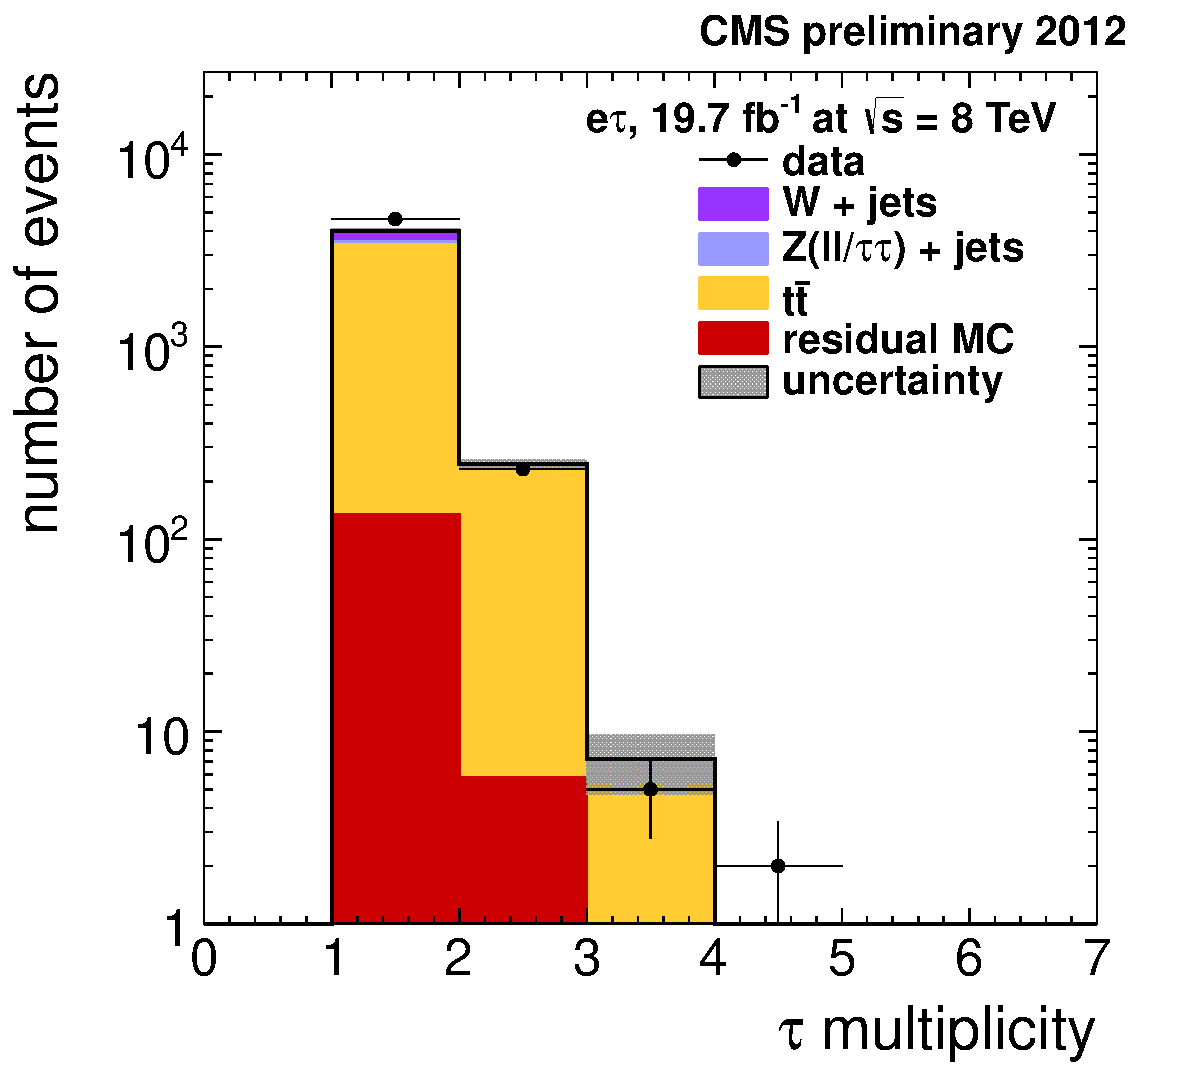
\includegraphics[width=0.49\textwidth]{figures/bkgEstim/ntauantiiso_etau_lqd321.pdf}
    \caption{Plots of the anti-isolated control region after the top squark final selection, showing the hadronic tau \pt spectrum (left) and multiplicity (right) in the \mutau channel (top) and the \etau channel (bottom). \label{Bkg:fig:antiiso-lqd321}}
  \end{center}
\end{figure}

The fake rate is used to weight the anti-isolated events in order to estimate the yield in the signal region. Because $f(\pt)$ is the probability for a fake hadronic tau candidate to be isolated, $1-f(\pt)$ is the probability for a fake hadronic tau candidate to fail isolation:
\begin{align}
P(\tau\text{ w/ given \pt is isolated}) &= f(\pt(\tau)), \\
P(\tau\text{ w/ given \pt is anti-isolated}) &= 1 - f(\pt(\tau)). \label{Bkg:eq:Pantiiso}
\end{align}
The signal region and the anti-isolated region are two complementary parts of a total region containing all events with hadronic tau candidates, passing or failing isolation. The probability that any given event in this total region is part of the anti-isolated region is equivalent to the probability that all hadronic taus in that event fail isolation. The isolation status of each tau in an event is independent, so this probability is given by the product of Eq. \eqref{Bkg:eq:Pantiiso} for each tau, shown in Eq. \eqref{Bkg:eq:Pantiisoall}. The signal region contains all events with at least one isolated hadronic tau. Therefore, the probability that an event in the total region is part of the signal region is given by the complement of the anti-isolated region probability, shown in Eq. \eqref{Bkg:eq:Piso1}.
\begin{align}
P(\text{all }\tau\text{s in event are anti-isolated}) &= \prod_{\tau}^{\text{(event)}}[1-f(\pt(\tau))] \label{Bkg:eq:Pantiisoall} \\
P(\text{at least 1 }\tau\text{ in event is isolated}) &= 1-\prod_{\tau}^{\text{(event)}}[1-f(\pt(\tau))] \label{Bkg:eq:Piso1}
\end{align}
Equation \eqref{Bkg:eq:faketauest} sums over all events in the anti-isolated region, using these complementary probabilities to produce a data-driven estimate of the major reducible background in the signal region.
\begin{equation} N_{\text{misID}~\tau} = \sum_{\text{events}}^{\text{(anti-iso)}} \frac{1 - \prod_{\tau}[1-f(\pt(\tau))]}{\prod_{\tau}[1-f(\pt(\tau))]} \label{Bkg:eq:faketauest} \end{equation}

Events in the signal region from the exclusive samples simulated for the \W + jets, \Z + jets, and \ttbar processes are used to predict the \ST distributions for the major reducible background. Because the dependency of the fake rate on \pt is similar in data and simulation, as shown in Fig. \ref{Bkg:fig:fakerate}, the simulated distributions are expected not to be biased with respect to the observed data. Only the events in which the leading selected hadronic tau is a misidentified jet, based on matching between reconstructed and generated particles, are considered. The simulated distributions are normalized to the data-driven estimation of the major reducible background yield.

In the leptoquark search, the central value for the yield estimation is calculated using the inclusive fake rate from the observed data and the observed events in the anti-isolated region. Systematic errors on this estimation are assigned based on variations in the fake rate and in the anti-isolated region. The inclusive fake rate is varied by the statistical uncertainty $\sigma_{\text{stat}}$ in both directions $f+1\sigma_{\text{stat}}$ and $f-1\sigma_{\text{stat}}$ separately for each bin. Each of the two variations is applied to the observed events in the anti-isolated region. The larger difference between the estimations from the two statistical variations and the central value is taken as a systematic uncertainty. Similarly, the $N_{\text{jet}} \geq 1$ fake rate from the observed data is applied to the observed events in the anti-isolated region, and the difference is taken as a systematic uncertainty. The contribution from residual backgrounds in the anti-isolated region is estimated using the inclusive fake rate from the observed data and included as an additional uncertainty. As mentioned previously, an uncertainty is also assessed due to the systematic difference in fake rates between \Zmm + jets events and semileptonic \ttbar events.

In the top squark search, the systematic uncertainties are computed in the same way. However, the central value for the yield estimation is calculated using the $N_{\text{jet}} \geq 1$ fake rate from the observed data, in order to account for the higher jet multiplicity. Correspondingly, the $N_{\text{jet}} \geq 2$ fake rate from the observed data is used as a variation. The overall systematic uncertainties are larger for both channels in the top squark search, compared to the leptoquark search. This is caused by the higher jet multiplicities required when calculating the fake rates in the \Zmm + jets control region, which reduces the number of events. In addition, the background in the top squark search is composed of a higher percentage of \ttbar events, which increases the contribution from the systematic deviation between the \Zmm + jets fake rate and the \ttbar fake rate.

Tables \ref{Bkg:tab:faketauresultsmutauLQ} and \ref{Bkg:tab:faketauresultsmutauLQD} show the results of the major reducible background estimation in the \mutau channel for the leptoquark search and the top squark search, respectively. The predictions from the simulation are in agreement with the data-driven values and with the closure test performed using the simulated fake rate and simulated anti-isolated events. These predictions are taken from \W + jets, \Z + jets, and \ttbar events in the signal region with matching between generated jets and reconstructed hadronic taus, normalized to $\lumi = \thelumi$. When contributions from all sources of systematic uncertainty are added in quadrature, the overall uncertainties are $16\%$ for the leptoquark search and $23\%$ for the top squark search. The statistical uncertainty from the anti-isolated region is approximately $1-2\%$ in all cases, which is negligible in comparison.

\begin{table}[hbt]
  \begin{center}
    \begin{tabular}{|c|c|r|r|}
      \multicolumn{4}{c}{\mutau channel} \\
      \hline
      \multicolumn{2}{|c|}{Sources} & \multicolumn{2}{c|}{LQ Results} \\
      \hline
      anti-iso      & fake rate                                           & \multicolumn{1}{c|}{yield}  & \multicolumn{1}{c|}{variation}\\
      \hline
      data          & data (incl.)                                        & 117.3 & (central)\\
      data          & data (incl.) ${}\pm 1\sigma_{\text{stat}}$          & 128.3 & 11.0 \\
      data          & data ($N_{\text{jet}} \geq 1$)                      & 106.5 & 10.7    \\
      residual bkg. & data (incl.)                                        & ---   & 7.0     \\
      \multicolumn{2}{|c|}{\Zmm vs. \ttbar fake rates ($18\%\times35\%$)} & ---   & 7.4 \\
      \hline
      \multicolumn{2}{|c|}{Final Result}         & \multicolumn{2}{c|}{$117.3 \pm 18.5$}\\
      \multicolumn{2}{|c|}{Simulated Prediction} & \multicolumn{2}{c|}{$117.7 \pm 28.7$}\\
      \multicolumn{2}{|c|}{Closure Test}         & \multicolumn{2}{c|}{$121.7 \pm \hphantom{1}3.5$}\\
      \hline
    \end{tabular}
    \caption{The results of the data-driven major reducible background estimation for the leptoquark search in the \mutau channel. This table shows all sources of systematic uncertainty and a comparison to the simulated prediction. Only statistical uncertainty is given for the simulated prediction and the closure test. From the two variations of the fake rate ${}\pm 1\sigma_{\text{stat}}$, the estimation with the larger difference from the central value is used.}
    \label{Bkg:tab:faketauresultsmutauLQ}
  \end{center}
\end{table}

\begin{table}[hbt]
  \begin{center}
    \begin{tabular}{|c|c|r|r|}
      \multicolumn{4}{c}{\mutau channel} \\
      \hline
      \multicolumn{2}{|c|}{Sources} & \multicolumn{2}{c|}{$\sTop$ Results} \\
      \hline
      anti-iso    & fake rate                                                    & \multicolumn{1}{c|}{yield}  & \multicolumn{1}{c|}{variation}\\
      \hline
      data        & data ($N_{\text{jet}} \geq 1$)                               & 59.8 & (central) \\
      data        & data ($N_{\text{jet}} \geq 1$) ${}\pm 1\sigma_{\text{stat}}$ & 67.0 & 7.2 \\
      data        & data ($N_{\text{jet}} \geq 2$)                               & 54.4 & 5.4     \\
      residual MC & data ($N_{\text{jet}} \geq 1$)                               & ---  & 2.1      \\
      \multicolumn{2}{|c|}{\Zmm vs. \ttbar fake rates ($18\%\times95\%$)}        & ---  & 10.2 \\
      \hline
      \multicolumn{2}{|c|}{Final Result}         & \multicolumn{2}{c|}{$59.8 \pm 13.8$}\\
      \multicolumn{2}{|c|}{Simulated Prediction} & \multicolumn{2}{c|}{$57.5 \pm \hphantom{1}6.5$} \\
      \multicolumn{2}{|c|}{Closure Test}         & \multicolumn{2}{c|}{$58.0 \pm \hphantom{1}1.3$} \\
      \hline
    \end{tabular}
    \caption{The results of the data-driven major reducible background estimation for the top squark search in the \mutau channel. This table shows all sources of systematic uncertainty and a comparison to the simulated prediction. Only statistical uncertainty is given for the simulated prediction and the closure test. From the two variations of the fake rate ${}\pm 1\sigma_{\text{stat}}$, the estimation with the larger difference from the central value is used.}
    \label{Bkg:tab:faketauresultsmutauLQD}
  \end{center}
\end{table}

In the \etau channel, there is a significant contribution from QCD events in the anti-isolated region. As described previously at the beginning of Sec. \ref{sec:faketaubkg}, the fake rate measured in the \Zmm + jets control region is not appropriate for QCD events. The QCD contribution must be subtracted from the major reducible background estimation calculated using the fake rate. Tables \ref{Bkg:tab:faketauresultsetauLQ} and \ref{Bkg:tab:faketauresultsetauLQD} show the results of the estimation in the \etau channel for the leptoquark search and the top squark search, respectively. The QCD contribution is already subtracted in these tables; the details of the subtraction will be discussed in Sec. \ref{sec:qcdbkg}. The sources of systematic uncertainty are the same as those considered in the \mutau channel, with an additional systematic uncertainty from the uncertainty on the subtracted QCD contribution. The results from the data-drive estimations are consistent with the simulated predictions and closure tests. The total uncertainty on the \etau channel yield is $17\%$ for the leptoquark search and $24\%$ for the top squark search.

\begin{table}[hbt]
  \begin{center}
    \begin{tabular}{|c|c|r|r|}
      \multicolumn{4}{c}{\etau channel} \\
      \hline
      \multicolumn{2}{|c|}{Sources} & \multicolumn{2}{|c|}{LQ Results} \\
      \hline
      anti-iso    & fake rate                                             & \multicolumn{1}{c|}{yield}  & \multicolumn{1}{c|}{variation} \\
      \hline
      data        & data (incl.)                                          & 124.2 & (central)   \\
      data        & data (incl.) ${}\pm 1\sigma_{\text{stat}}$            & 138.5 & 14.3 \\
      data        & data ($N_{\text{jet}} \geq 1$)                        & 113.9 & 10.3         \\ 
      residual MC & data (incl.)                                          & ---   & 7.1              \\
      QCD         & data (incl.)                                          & ---   & 2.7  \\
      \multicolumn{2}{|c|}{\Zmm vs. \ttbar fake rates ($18\%\times35\%$)} & --- & 7.8 \\
      \hline
      \multicolumn{2}{|c|}{Final Result}         & \multicolumn{2}{c|}{$124.2 \pm 20.7$} \\
      \multicolumn{2}{|c|}{Simulated Prediction} & \multicolumn{2}{c|}{$106.8 \pm 27.3$} \\
      \multicolumn{2}{|c|}{Closure Test}         & \multicolumn{2}{c|}{$129.5 \pm \hphantom{1}3.6$} \\
      \hline
    \end{tabular}
    \caption{The results of the data-driven major reducible background estimation for the leptoquark search in the \etau channel. This table shows all sources of systematic uncertainty and a comparison to the simulated prediction. Only statistical uncertainty is given for the simulated prediction and the closure test. From the two variations of the fake rate ${}\pm 1\sigma_{\text{stat}}$, the estimation with the larger difference from the central value is used.}
    \label{Bkg:tab:faketauresultsetauLQ}
  \end{center}
\end{table}

\begin{table}[hbt]
  \begin{center}
    \begin{tabular}{|c|c|r|r|}
      \multicolumn{4}{c}{\etau channel} \\
      \hline
      \multicolumn{2}{|c|}{Sources} & \multicolumn{2}{|c|}{$\sTop$ Results} \\
      \hline
      anti-iso    & fake rate                                                  & \multicolumn{1}{c|}{yield}  & \multicolumn{1}{c|}{variation} \\
      \hline
      data        & data ($N_{\text{jet}} \geq 1$)                               & 65.7 & (central) \\
      data        & data ($N_{\text{jet}} \geq 1$) ${}\pm 1\sigma_{\text{stat}}$ & 74.6 & 8.9 \\
      data        & data ($N_{\text{jet}} \geq 2$)                               & 59.8 & 5.9   \\
      residual MC & data ($N_{\text{jet}} \geq 1$)                               & ---  & 1.8      \\
      QCD         & data ($N_{\text{jet}} \geq 1$)                               & ---  & 0.1 \\
      \multicolumn{2}{|c|}{\Zmm vs. \ttbar fake rates ($18\%\times95\%$)}        & ---  & 11.2 \\
      \hline
      \multicolumn{2}{|c|}{Final Result}         & \multicolumn{2}{c|}{$65.7 \pm 15.6$}\\
      \multicolumn{2}{|c|}{Simulated Prediction} & \multicolumn{2}{c|}{$66.7 \pm \hphantom{1}7.6$} \\
      \multicolumn{2}{|c|}{Closure Test}         & \multicolumn{2}{c|}{$61.6 \pm \hphantom{1}1.4$} \\
      \hline
    \end{tabular}
    \caption{The results of the data-driven major reducible background estimation for the top squark search in the \etau channel. This table shows all sources of systematic uncertainty and a comparison to the simulated prediction. Only statistical uncertainty is given for the simulated prediction and the closure test. From the two variations of the fake rate ${}\pm 1\sigma_{\text{stat}}$, the estimation with the larger difference from the central value is used.}
    \label{Bkg:tab:faketauresultsetauLQD}
  \end{center}
\end{table}

\subsubsection{QCD Multijet Reducible Background}
\label{sec:qcdbkg}

The estimation of the contribution from the QCD multijet process in the \etau channel requires two steps. The presence of QCD events in the observed data in the \etau anti-isolated control region biases the previous estimation, as these events are weighted by the inappropriate quark-jet fake rate. Therefore, the first step must be to estimate the yield and \pt distribution of the QCD events in the anti-isolated observed data, in order to correct that bias by subtracting the inappropriate portion of the fake rate estimation. The second step is to perform an independent estimation of the QCD contribution in the signal region using the observed data.

In both steps, a same-sign/opposite-sign (SS/OS) method is used to estimate the number of QCD events in a given region of the data. A same-sign control region is defined by requiring that the light lepton and hadronic tau have the same electric charge, instead of the opposite charge. Because both objects are misidentified jets in QCD events, their charge assignments are expected to be random, so the number of events in which both objects have the same charge should be the same as for the opposite charge. In practice, a slight deviation between the numbers of same-sign and opposite-sign events is possible, for example due to charge asymmetries in proton-proton collisions. The scale factor relating the numbers of same-sign and opposite-sign events was measured to be 1.06 in Ref. \cite{CMS-AN-2013-178}.

The non-QCD background in the same-sign control region is estimated using the simulation and subtracted from the observed data; any remaining events are assumed to originate from the QCD process. The scale factor of 1.06 is applied to extrapolate from this yield $N_{\text{QCD}}^{\text{SS}}$ to the opposite-sign region $N_{\text{QCD}}^{\text{OS}}$:
\begin{align}
N_{\text{QCD}}^{\text{SS}} & = N_{\text{data}}^{\text{SS}} - N_{\text{MC}}^{\text{SS}}, \label{bkg:QCDss}\\
N_{\text{QCD}}^{\text{OS}} & = 1.06 N_{\text{QCD}}^{\text{SS}}. \label{bkg:QCDos}
\end{align}
The subtraction of non-QCD backgrounds can potentially involve a large number of events. In order to ensure the validity of the subtraction, the normalization of the simulated samples must be carefully checked.

To check the normalization of the simulated \W + jets, \Zll, and \Ztt samples, a region of data is defined using the preselection criteria without the cut $N_{\text{jets}}\geq2$. Most of the events at the preselection level are eventually eliminated from the signal region by the stricter main and final selections, so the contents of the signal region make up a relatively small portion of this larger region. The transverse mass of the electron and \met system, $\MT(\Pe,\met)$, is defined in Eq. \eqref{eq:MTdef}:
\begin{equation}
\MT(\Pe,\met) = \sqrt{2\pt^{(\Pe)}\met\left[1-\text{cos}\left(\Delta\phi\left(\Pe,\met\right)\right)\right]}. \label{eq:MTdef}
\end{equation}
This definition assumes both particles in the system are massless, which is a good approximation for highly relativistic electrons and neutrinos. The \MT distribution in the region defined above is used to determine normalization parameters for the simulated samples by comparing them to the observed data:
\begin{equation}
\MT^{\text{(data)}} = r_{\W}\MT^{\text{(\W + jets)}} + r_{\tau}\MT^{(\Ztt)} + r_{\ell}\MT^{(\Zll)} + \MT^{\text{(\ttbar,\cPqt,VV)}}. \label{Bkg:eq:MTmin}
\end{equation}
The difference between the sum of the simulated \MT distributions and the observed \MT distribution is minimized by varying the three normalization parameters $r_{\W}$, $r_{\tau}$, and $r_{\ell}$. The normalization of the other processes, \ttbar, single top, and diboson, is not addressed in this minimization. The observed distribution contains a contribution from QCD which is not modeled in the simulation. Therefore, at least one of the normalization parameters will be inflated during the minimization in order to include this contribution. Measurements of the inclusive \W and \Z production cross sections have demonstrated a similarity between the \MT distributions for \Zll and QCD events when using a selection tuned for \Wln events \cite{CMS-AN-2010-359,CMS:2011aa}. Hypothesizing that this similarity holds for the selection considered here, the parameter $r_{\ell}$ should scale the simulated \Zll yield to include the QCD yield.

The minimization in Eq. \eqref{Bkg:eq:MTmin} provides the following values for the $r$ parameters: $r_{W} = 0.86$, $r_{\tau} = 1.21$, $r_{\ell} = 2.02$. Using these parameters, corrected yields $N$ can be defined for the simulated samples, based on the uncorrected yields $N_{\text{MC}}$:
\begin{align}
N(\text{\W + jets}) &= r_{\W}N_{\text{MC}}(\text{\W + jets}), \\
N(\Ztt) &= r_{\tau}N_{\text{MC}}(\text{\Ztt}), \\
N(\Zll) + N(\text{QCD}) &= r_{\ell}N_{\text{MC}}(\text{\Zll}). \label{Bkg:eq:NZllQCD}
\end{align}
Equation \eqref{Bkg:eq:NZllQCD} arises from the hypothesis that the \Zll yield will be scaled to include the QCD yield. This can be used to check the validity of the \MT minimization method for correcting the simulated sample normalizations. The parameter $r_{\tau}$ is assigned to be the normalization correction for both the \Zll and \Ztt samples, in order to solve for $N(\text{QCD})$ in terms of known quantities:
\begin{align}
N(\Zll) &= r_{\tau}N_{\text{MC}}(\text{\Zll}), \label{eq:NZll} \\
N(\text{QCD}) &= r_{\ell}N_{\text{MC}}(\text{\Zll}) - r_{\tau}N_{\text{MC}}(\text{\Zll}). \label{eq:NQCDZ}
\end{align}
Equation \eqref{eq:NQCDZ} follows from the combination of Eqs. \eqref{Bkg:eq:NZllQCD} and \eqref{eq:NZll}. This equation produces the value $N(\text{QCD}) = 24765 \pm 1411$ for the region defined by the preselection criteria without the cut $N_{\text{jets}}\geq2$. In comparison, the SS/OS method applied directly to this region predicts the value $N(\text{QCD}) = 26424 \pm 1250$. These two values agree within uncertainties, validating the assumptions made in the \MT minimization method. The normalization parameters $r_{\W}$ and $r_{\tau}$ will be used for the \W + jets and \Z + jets normalizations in the various same-sign and anti-isolated control regions necessary to conduct the two steps of the QCD estimation in the signal region. A separate control region requiring $N_{\text{b-jet}}\geq2$ and $\MT>70\GeV$ is used to check the normalization of the \ttbar simulation, and no correction is found to be necessary.

To measure the QCD portion of the observed data in the anti-isolated region, the SS/OS method described by Eqs. \eqref{bkg:QCDss} and \eqref{bkg:QCDos} is applied, using the normalization parameters. Figure \ref{fig:QCDSSAiso} shows the \MT(\Pe,\met) distribution in the same-sign anti-isolated control region for the leptoquark search, with an overall excess in the observed data indicating the presence of QCD. This method predicts $3026\pm210$ QCD events after the leptoquark final selection and $152\pm15$ events after the top squark final selection. In order to subtract these events' contribution from the reducible background estimation, the \pt distribution of the hadronic tau candidates in the QCD events is needed. Figure \ref{Bkg:fig:antiiso} shows that the QCD events in the \etau anti-isolated region are found primarily in the single tau multiplicity bin. Therefore, it is sufficient to subtract the simulated tau \pt distribution from the observed tau \pt distribution to obtain the QCD tau \pt distribution. A simplified version of Eq. \eqref{Bkg:eq:faketauest} can be used to weight these single-tau events:
\begin{equation}
N_{\text{misID}~\tau}^{\text{(QCD)}} = N_{\text{anti-iso}}^{\text{(QCD)}} \sum_{\pt}{\frac{f(\pt)}{1-f(\pt)}}. \label{Bkq:eq:faketausubQCD}
\end{equation}
Using Eq. \eqref{Bkq:eq:faketausubQCD}, the QCD yield to subtract is found to be $38.5\pm2.7$ events in the leptoquark search and $1.5\pm0.1$ events in the top squark search. The subtraction of these QCD yields is already included in the results shown in Tables \ref{Bkg:tab:faketauresultsetauLQ} and \ref{Bkg:tab:faketauresultsetauLQ}, with the statistical uncertainties on the QCD yields included as additional systematic uncertainties on the final major reducible background estimation.

\begin{figure}[hbt]
  \begin{center}
    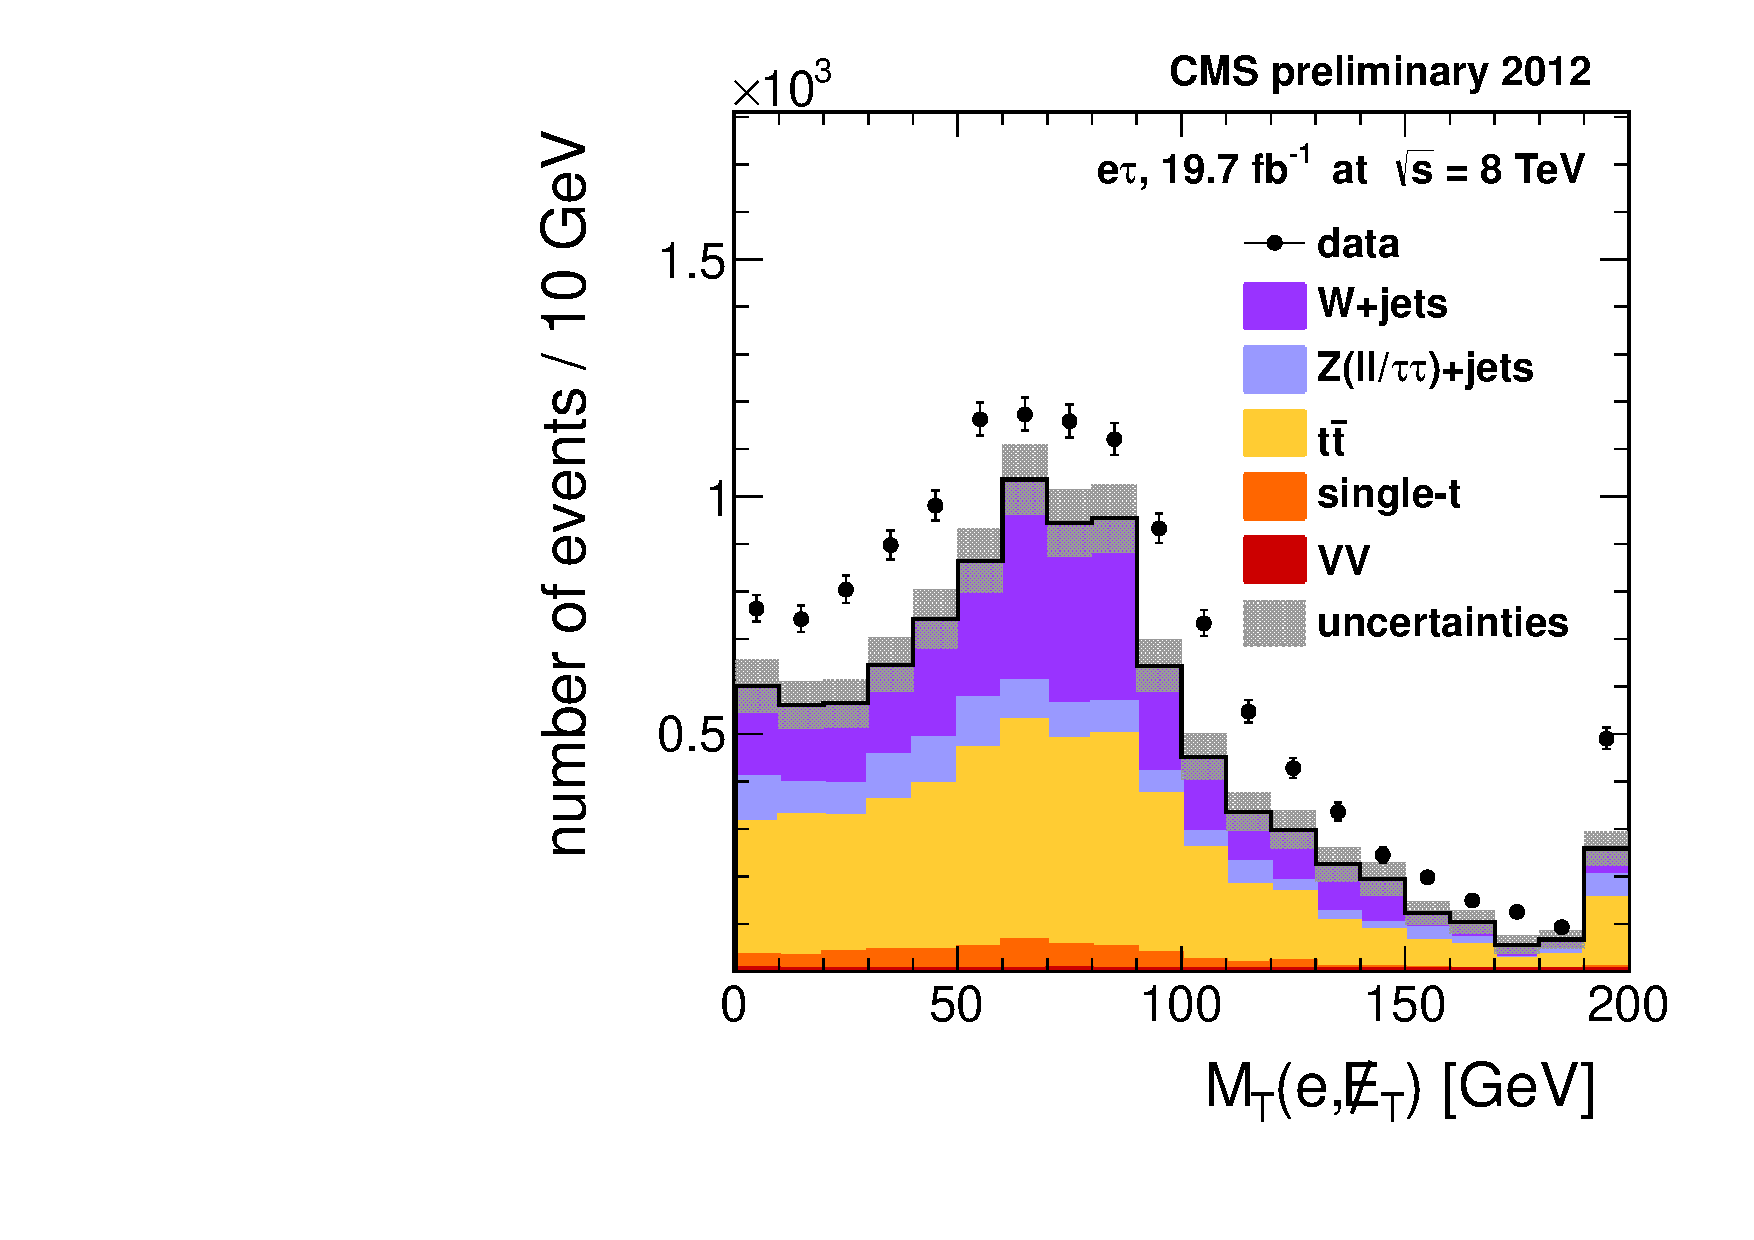
\includegraphics[width=0.6\textwidth]{figures/etau/eMETTMassSSAIsoFinal.pdf}
    \caption{The transverse mass of the electron and missing transverse energy system for the same-sign anti-isolated control region, after the leptoquark final selection. The overall excess in the observed data, not localized in a specific range of \MT values, indicates the presence of QCD events.}
    \label{fig:QCDSSAiso}
  \end{center}
\end{figure}

Having subtracted the improperly estimated QCD contribution, the actual contribution from QCD, if any, must be obtained. Again, the SS/OS method is used, now with the signal region. To decrease the statistical uncertainty in this estimation, the same-sign control region is defined before the final selection. For the leptoquark search, this means that the cut $\MassTJ>250\GeV$ is not applied. Figure \ref{fig:QCDSSMET} shows the \met distribution in this control region, with an excess in the observed data at low \met indicating the presence of QCD. Using the normalization corrections derived previously, the simulated yield in this control region is found to be $474\pm18$ events, while the observed yield is found to be $736\pm27$, which gives $N_{\text{QCD}}^{\text{SS}} = 262\pm32$ and correspondingly $N_{\text{QCD}}^{\text{OS}} = 277\pm34$. To extrapolate this QCD yield to the region defined by the leptoquark final selection, the efficiency of the cut $\MassTJ>250\GeV$ is measured in a same-sign control region which vetoes events containing one or more b-tagged jets, enhancing the contribution from QCD. The QCD yields before and after the mass cut are defined as the subtraction of the simulated yields from the observed yields:
\begin{alignat}{8}
N_{\text{QCD}}^{\text{before}} &= N_{\text{data}}^{\text{before}} &&- N_{\text{MC}}^{\text{before}} &&= (793 &&\pm 28) &&- (469 &&\pm 19) &&= 324 &&\pm 34, \\
N_{\text{QCD}}^{\text{after}} &= N_{\text{data}}^{\text{after}}   &&- N_{\text{MC}}^{\text{after}}  &&= (\hphantom{7}93  &&\pm 10) &&- (\hphantom{4}66  &&\pm \hphantom{1}7)  &&= \hphantom{3}27  &&\pm 12.
\end{alignat}
The ratio of these two yields is the efficiency of the cut, $\varepsilon_{\MassTJ}=8.5\%\pm4.0\%$. Thus, Eq. \eqref{eq:NQCDfinal} calculates the final yield from QCD in the leptoquark search:
\begin{equation}
N_{\text{QCD}}^{\text{final}} = N_{\text{QCD}}^{\text{OS}} \times \varepsilon_{\MassTJ} = (277\pm 34) \times (8.5\% \pm 4\%) = 23.6 \pm 12. \label{eq:NQCDfinal}
\end{equation}
To check this estimation, the SS/OS method is applied to the signal region after the cut $\MassTJ>250\GeV$. This check gives a less precise result $N_{\text{QCD}}^{\text{SS/OS}} = 31.8 \pm 21.2$, which is fully compatible with the above result within uncertainties.

\begin{figure}[hbt]
  \begin{center}
    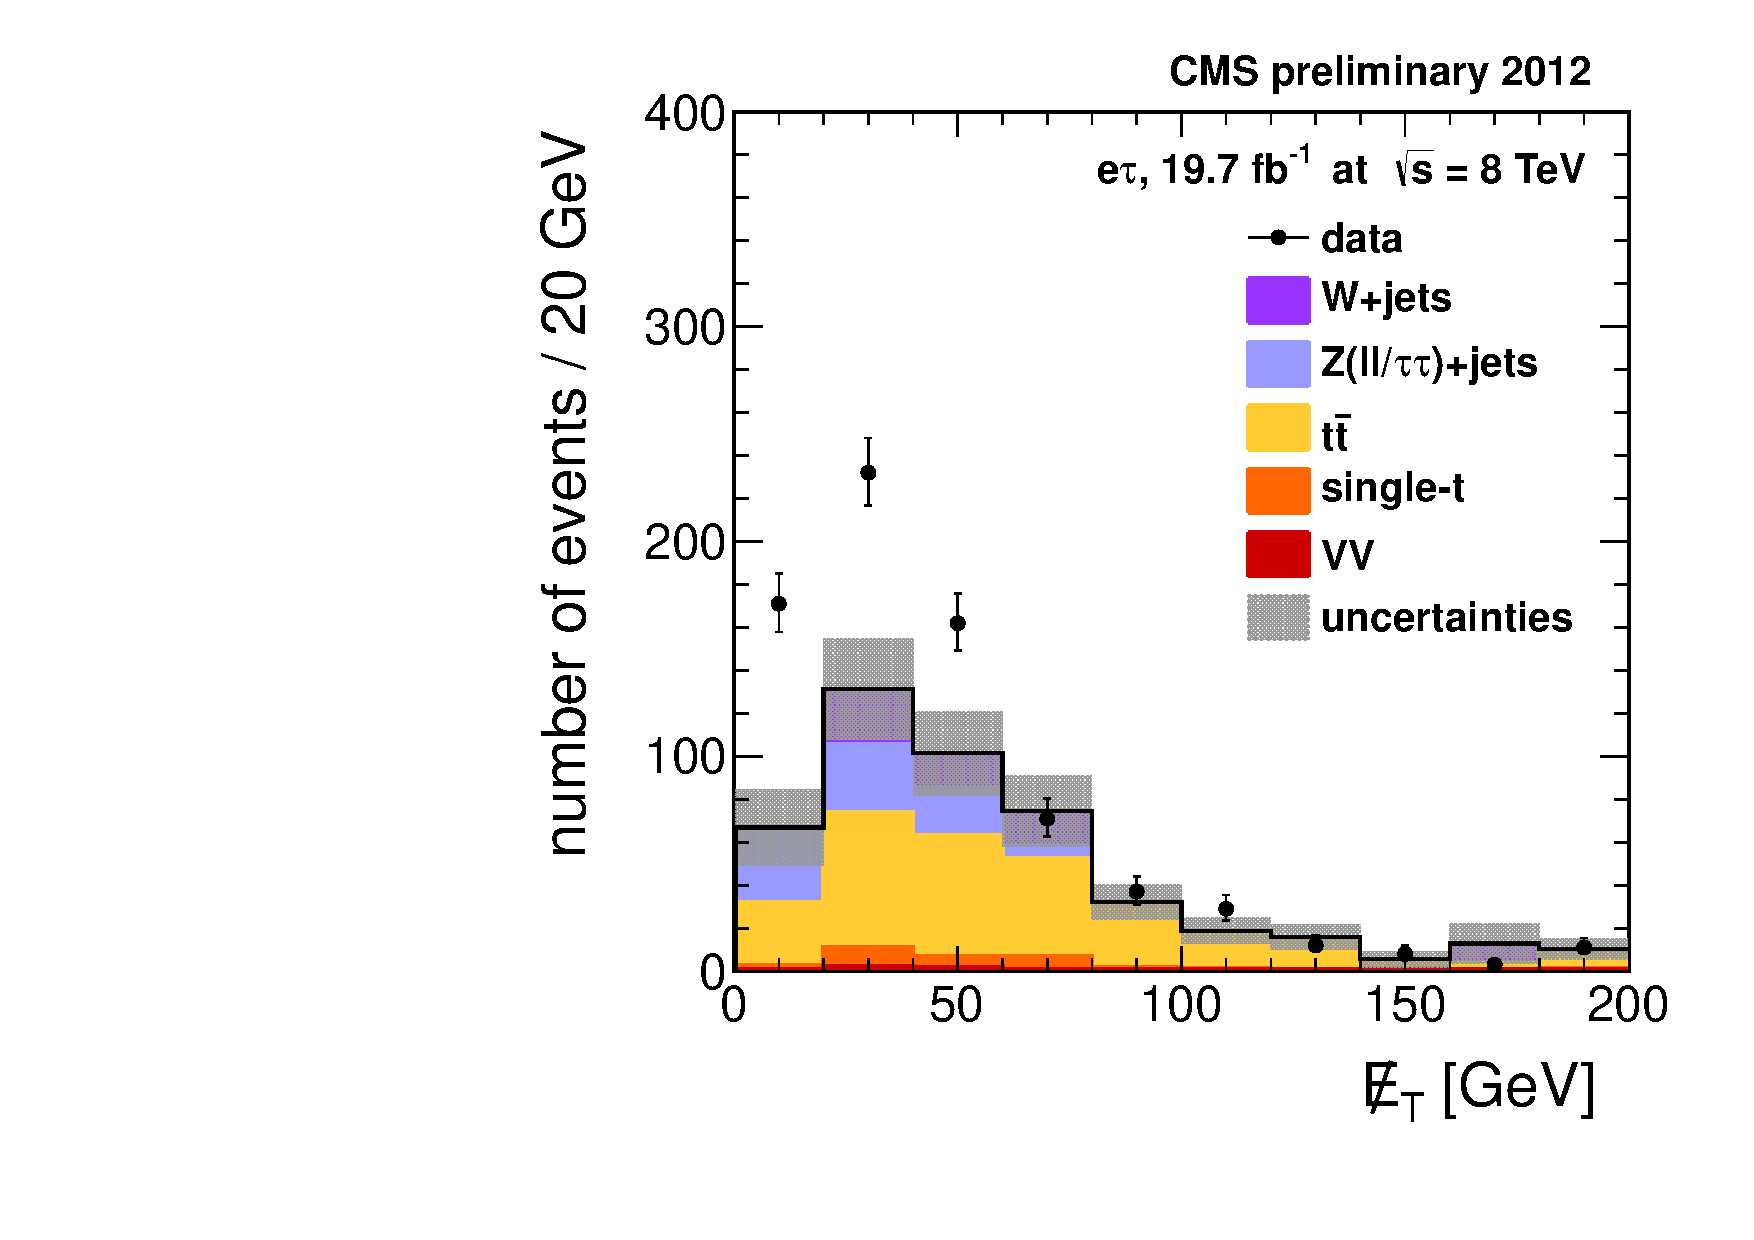
\includegraphics[width=0.6\textwidth]{figures/etau/metPtSSIso.pdf}
    \caption{The missing transverse energy spectrum for the same-sign control region selected before the $\MassTJ>250\GeV$ requirement for the leptoquark search. The excess of observed events at low \met is an indication of the presence of QCD events.}
    \label{fig:QCDSSMET}
  \end{center}
\end{figure}

In addition to the yield, the \ST distribution for the QCD process has to be estimated from the observed data, as no simulated sample is available to produce it. The distribution is obtained by subtracting the simulated \ST distribution from the observed \ST distribution in the same-sign control region after the full leptoquark final selection, as shown in Fig. \ref{fig:residQCD}. The bins with negative values, all of which are equivalent to zero within their statistical uncertainties, are set to be zero to avoid unphysical values in the distribution. The QCD \ST distribution obtained from this method is then added to the major reducible \ST distribution for the \etau channel. The propagated statistical uncertainty on the QCD yield, $\pm 12$ events, is added in quadrature with the systematic uncertainty from the major reducible background estimation.

\begin{figure}[hbt]
  \begin{center}
    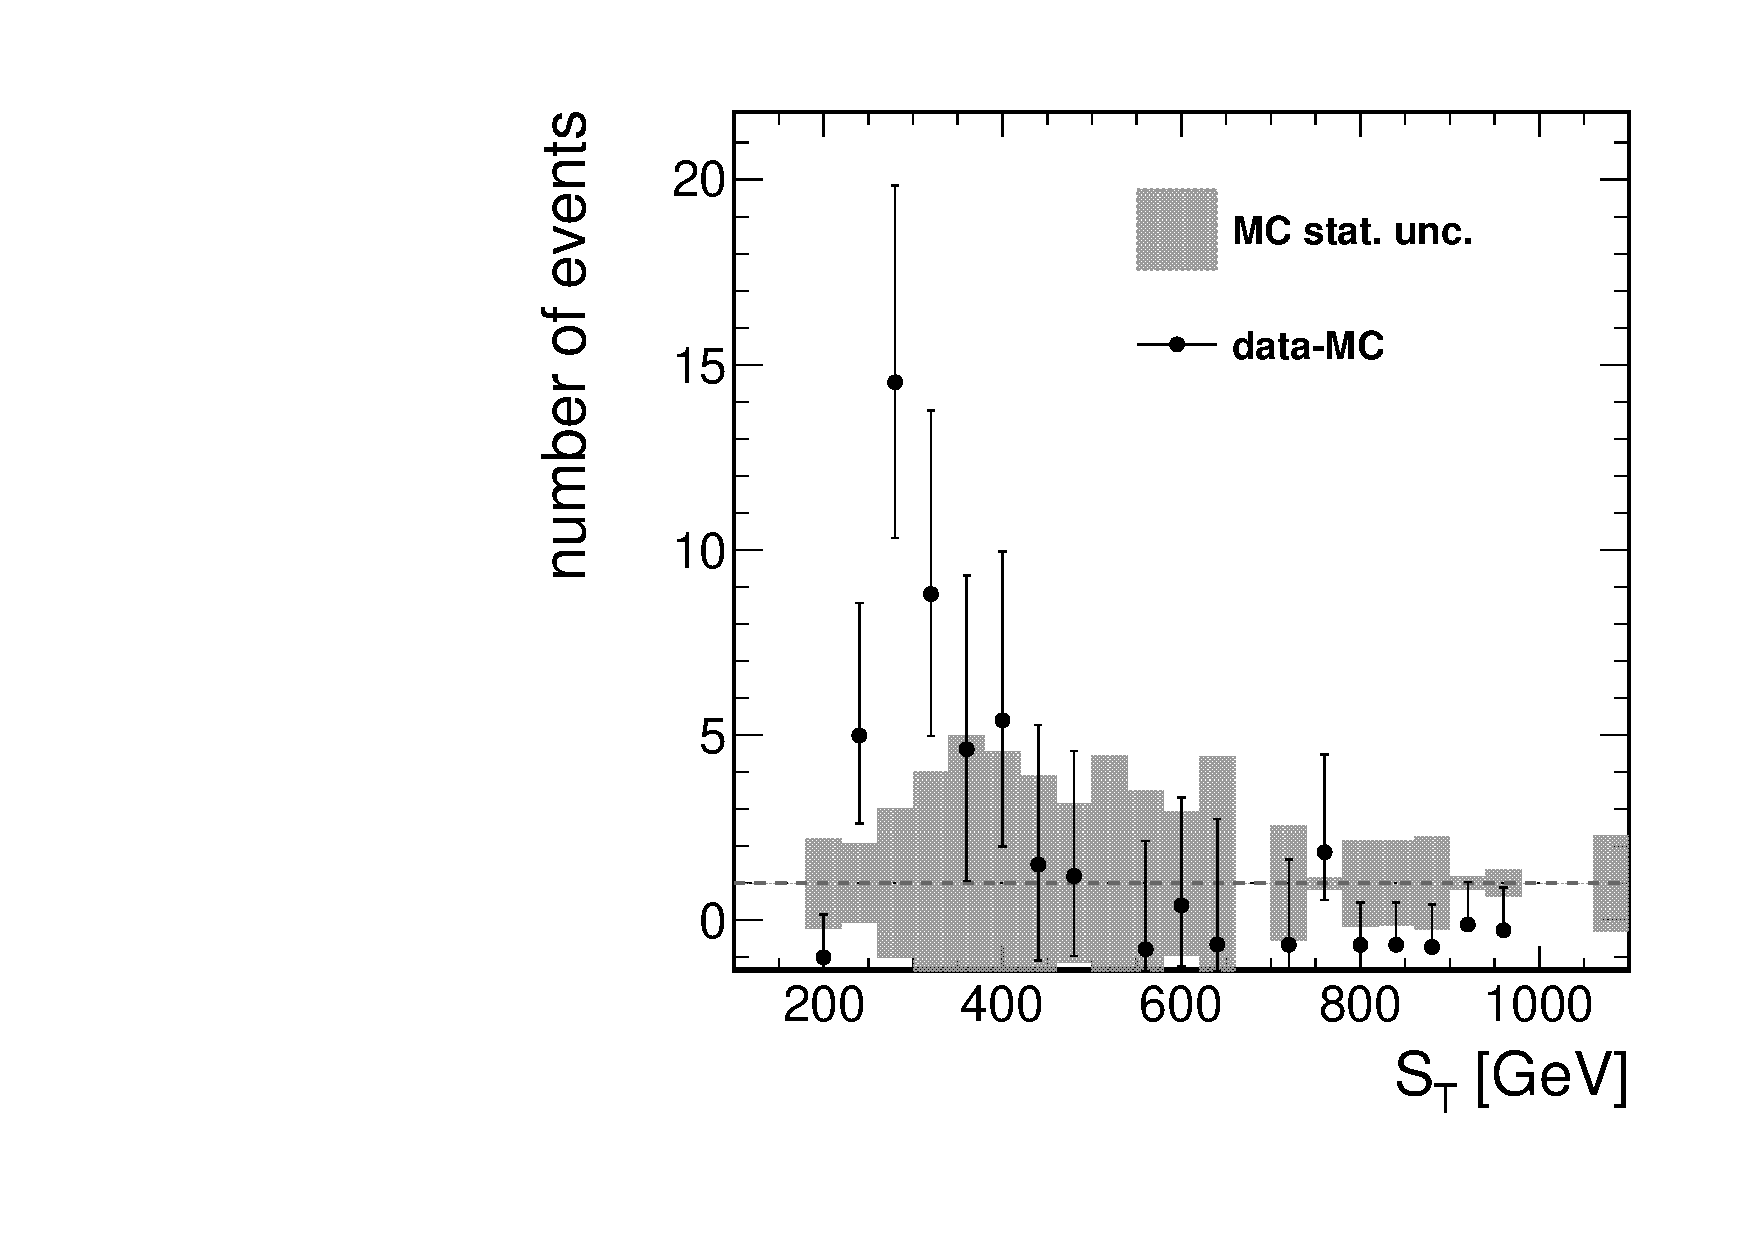
\includegraphics[width=0.6\textwidth]{figures/bkgEstim/residualQCD.pdf}
    \caption{The QCD \ST distribution estimated by subtracting the simulated distribution from the observed distribution in the same-sign control region after the leptoquark final selection. The negative values are set to zero when using the distribution.}
    \label{fig:residQCD}
  \end{center}
\end{figure}

In the top squark search, the QCD background is found to be $0 \pm 13$ using the SS/OS method with an extrapolation of the efficiency of the cut $N_{\text{jets}}\geq5$. Applying the SS/OS method after the final selection to check that prediction finds $0 \pm 18$. These predictions agree and are both equivalent to zero events, so no QCD background is added to the \etau channel in the top squark search. This lack of QCD background is expected due to the high jet multiplicity requirement in this selection.
